% !TeX program = lualatex
% !TeX spellcheck = uk_UA

\documentclass[14pt, a4paper]{extarticle}

% -- Мови та шрифти (згідно з ДСТУ) --
\usepackage{fontspec}
\usepackage[english, ukrainian]{babel}
\usepackage{csquotes}

\setmainfont{Times New Roman}
\setsansfont{Arial}
\setmonofont{Courier New}[Scale=0.85]

% -- Математичні пакети --
\usepackage{amsmath, amssymb, mathtools}

% -- Оптимізація тексту для LuaLaTeX --
\usepackage[protrusion=true, expansion=true]{microtype}
\emergencystretch=3.5em
\hbadness=10000

% -- Параметри сторінки згідно з ДСТУ 3008:2015 --
\usepackage[
    left=30mm,
    right=15mm,
    top=20mm,
    bottom=20mm,
    footskip=10mm,
    headheight=17pt
]{geometry}

% -- Міжрядковий інтервал (еквівалент 1.5 Word) та абзацний відступ --
\linespread{1.3}
\usepackage{indentfirst}
\setlength{\parindent}{1.25cm}
\setlength{\parskip}{0pt}

% -- Колонтитули та нумерація сторінок (вгорі праворуч, без лінійок) --
\usepackage{fancyhdr}
\fancypagestyle{plain}{
    \fancyhf{}
    \rhead{\thepage}
    \renewcommand{\headrulewidth}{0pt}
}
\pagestyle{plain}

% -- Форматування заголовків згідно з ДСТУ 3008:2015 --
\usepackage[explicit]{titlesec}

% Формат розділів (14pt, напівжирний, абзацний відступ 1.25cm)
\titleformat{\section}[block]
{\normalsize\bfseries\raggedright}
{\thesection\ }
{0pt}
{#1}
\titlespacing*{\section}{\parindent}{14pt}{7pt}

% Формат підрозділів
\titleformat{\subsection}[block]
{\normalsize\bfseries\raggedright}
{\thesubsection\ }
{0pt}
{#1}
\titlespacing*{\subsection}{\parindent}{14pt}{7pt}

% -- Списки (компактні, вирівняні за абзацним відступом) --
\usepackage{enumitem}
\setlist{
    nosep,
    leftmargin=*,
    labelindent=\parindent
}
\setlist[itemize]{label=--}

% -- Підписи до рисунків та таблиць згідно з ДСТУ 3008:2015 --
\usepackage{caption}
\DeclareCaptionLabelSeparator{emdash}{ — }

\captionsetup[figure]{
    labelsep=emdash,
    name={Рисунок},
    justification=centering,
    position=bottom,
    font=normalsize
}

\captionsetup[table]{
    labelsep=emdash,
    name={Таблиця},
    justification=raggedright,
    singlelinecheck=false,
    position=top,
    font=normalsize
}

% -- Таблиці (книжковий стиль, нормальний інтервал) --
\usepackage{booktabs}
\renewcommand{\arraystretch}{1.0}

% -- Графіка та гіперпосилання --
\usepackage{graphicx}
\usepackage[hidelinks]{hyperref}

% -- Завантаження модуля обробки таблиць Lua --
\directlua{dofile("tables.lua")}

\begin{document}

% -- Титульна сторінка --
\begin{titlepage}
    \thispagestyle{empty}
    \setlength{\parindent}{0pt}
    
    % -- ШАПКА ДОКУМЕНТА (12pt, напівжирний) --
    \begin{center}
        {\fontsize{12pt}{16pt}\selectfont\bfseries
        МІНІСТЕРСТВО ОСВІТИ І НАУКИ УКРАЇНИ\\[3pt]
        ОДЕСЬКИЙ НАЦІОНАЛЬНИЙ УНІВЕРСИТЕТ ІМЕНІ І.І. МЕЧНИКОВА\\[3pt]
        ФАКУЛЬТЕТ МАТЕМАТИКИ, ФІЗИКИ ТА ІНФОРМАЦІЙНИХ ТЕХНОЛОГІЙ\\[3pt]
        КАФЕДРА ОПТИМАЛЬНОГО КЕРУВАННЯ ТА ЕКОНОМІЧНОЇ КІБЕРНЕТИКИ\par}
    \end{center}

    \vspace{1.5cm}

    % -- НАЗВА РОБОТИ ТА ТЕМА --
    \begin{center}
        {\fontsize{18pt}{22pt}\selectfont\bfseries ЗВІТ\\
        до лабораторної роботи № 4\par}
        \vspace{0.4cm}
        {\fontsize{14pt}{18pt}\selectfont
        з дисципліни «Системи комп’ютерного зору»\par}
        \vspace{0.4cm}
        {\fontsize{16pt}{20pt}\selectfont\bfseries
        на тему:\\[6pt]
        «Зіставлення ознак, RANSAC, побудова панорами»\par}
    \end{center}

    \vspace{1.5cm}

    % -- ПРАВИЙ БЛОК (Виконавець) --
    \hfill
    \begin{minipage}{0.60\textwidth}
        \raggedright
        {\fontsize{14pt}{19pt}\selectfont
        Виконав:\\[2pt]
        студент 3 курсу групи 1\\[2pt]
        спеціальності F1 «Прикладна математика»\\[2pt]
        Касьянов Ярослав Володимирович
        }
    \end{minipage}

    \vfill

    % -- МІСТО ТА РІК --
    \begin{center}
        {\fontsize{12pt}{14pt}\selectfont\bfseries Одеса -- 2026\par}
    \end{center}
\end{titlepage}

% За ДСТУ титульна сторінка входить у загальну нумерацію як 1-ша, 
% тому наступна сторінка отримує номер 2:
\setcounter{page}{2}



\section{Мета роботи}
Теоретичне та експериментальне вивчення методів зіставлення локальних геометричних ознак (feature matching) у комп'ютерному зорі; дослідження поведінки критерію відношення відстаней Лоу (Lowe's ratio test) та симетричної взаємної перевірки (cross-check); дослідження критичної нестійкості класичного методу найменших квадратів (МНК) до викидів при оцінці проєктивної гомографії; самостійна покрокова алгоритмічна реалізація робастного методу узгодження випадкових вибірок (RANSAC) із контролем невиродженості 4-точкових конфігурацій; порівняння теоретичної оцінки кількості ітерацій, фіксованого бюджету та адаптивного критерію зупинки на серії незалежних запусків; дослідження залежності об'єму консенсусної множини та похибки репроєкції від порога узгодженості $\tau$; побудова безшовної панорами плоскої сцени з 5 кадрів із ланцюговим множенням гомографій та лінійним ваговим блендуванням у зонах перекриття; аналіз типових випадків відмови (дефіцит перекриття з виродженням проєктивної геометрії та просторовий паралакс при зйомці тривимірної сцени зі зміщенням центра проєкції).

\section{Вихідні дані}
\begin{itemize}
    \item \textbf{Апаратне забезпечення}: смартфон Google Pixel 5. Основний фотомодуль: фокусна відстань $f = 4.38$~мм ($27$~мм в еквіваленті 35-мм плівки), світлосила об'єктива $f/1.73$, оптичний CMOS-сенсор формату $1/2.55''$ (фізичний розмір пікселя $1.4 \times 1.4$~мкм).
    \item \textbf{Тестові набори власних зображень}:
    \begin{itemize}
        \item \textbf{Набір предметної сцени з жорстким диском (каталог \texttt{Homework}, $4032 \times 2268$~пк)}: серії ракурсів \texttt{angle1}--\texttt{angle10} та масштабів \texttt{scale1}--\texttt{scale5}. Для детального аналізу зіставлення ознак, чутливості МНК та поведінки RANSAC (Частини A, B, C) використано пару сусідніх кадрів \texttt{angle4}--\texttt{angle5} ($28624$ і $12182$ SIFT-точок; проєкція \texttt{angle4} покриває $69.4\%$ площі \texttt{angle5}, при цьому в кадрі \texttt{angle5} видимі $93.0\%$ площі \texttt{angle4}) та пару зі зміною масштабу \texttt{scale3}--\texttt{scale4} ($53341$ і $9793$ SIFT-точок; кадр \texttt{scale3} повністю вкладений у \texttt{scale4} та покриває $41.4\%$ його площі, що відповідає умові практикуму про перекриття $\approx 40\%$). Оскільки серія \texttt{angle1}--\texttt{angle10} знята обходом камери зі зміщенням оптичного центра навколо рельєфного 3D-об'єкта (корпус HDD висотою $26$~мм на столі та клавіатура на задньому плані), у Частині E послідовність \texttt{angle2}--\texttt{angle6} використана для кількісної та візуальної демонстрації оптичного паралаксу, а пари з рознесеними ракурсами (\texttt{angle2}--\texttt{angle5}, \texttt{angle4}--\texttt{angle8}, \texttt{angle8}--\texttt{angle10}) і стрибком масштабу (\texttt{scale1}--\texttt{scale5}) -- для аналізу відмови при дефіциті перекриття.
        \item \textbf{Планарна серія для побудови панорами (каталог \texttt{corners}, оригінал $4032 \times 3024$~пк, робочий масштаб $0.5$: $2016 \times 1512$~пк)}: 5 послідовних кадрів плоскої сцени (шахова дошка, зафіксована монетами на дерев'яній площині) \texttt{corner\_7}, \texttt{corner\_6}, \texttt{corner\_4}, \texttt{corner\_5}, \texttt{corner\_3} з центральним опорним кадром \texttt{corner\_4} (Частина D). Оскільки об'єкти сцени лежать в одній фізичній площині, проєктивна гомографія між кадрами є математично точною незалежно від трансляції камери.
    \end{itemize}
\end{itemize}

\section{Теоретичні відомості}
\begin{enumerate}
    \item \textbf{Проєктивна гомографія}: для однорідних координат відповідних точок $p_1 = (x_1, y_1, 1)^T$ та $p_2 = (x_2, y_2, 1)^T$ двох зображень плоскої сцени (або довільної 3D-сцени при чистому обертанні камери навколо оптичного центра) геометричне відображення задається невиродженою матрицею $H \in \mathbb{R}^{3 \times 3}$ з точністю до ненульового множника ($8$ ступенів вільності):
    \begin{equation}\label{eq:homography_hom}
        p_2 \sim H p_1 \iff 
        \begin{pmatrix} x_2 \\ y_2 \\ 1 \end{pmatrix} \sim 
        \begin{pmatrix} h_{11} & h_{12} & h_{13} \\ h_{21} & h_{22} & h_{23} \\ h_{31} & h_{32} & h_{33} \end{pmatrix}
        \begin{pmatrix} x_1 \\ y_1 \\ 1 \end{pmatrix}.
    \end{equation}
    У декартівських координатах точкове відображення $\hat{p}_2 = \pi(H p_1)$ має вигляд:
    \begin{equation}\label{eq:homography_cart}
        \hat{x}_2 = \frac{h_{11} x_1 + h_{12} y_1 + h_{13}}{h_{31} x_1 + h_{32} y_1 + h_{33}}, \quad
        \hat{y}_2 = \frac{h_{21} x_1 + h_{22} y_1 + h_{23}}{h_{31} x_1 + h_{32} y_1 + h_{33}}.
    \end{equation}
    Геометрично коректна гомографія повинна зберігати додатність проєктивного знаменника $w_i = h_{31} x_i + h_{32} y_i + h_{33} > 0$ для всіх чотирьох кутів кадру (відсутність перетину «лінії горизонту») та переводити прямокутник кадру в опуклий чотирикутник із розумним відношенням площ.

    \item \textbf{Критерій відношення відстаней Лоу (Lowe's ratio test)}: для дескриптора $d_1$ та двох його найближчих сусідів $d_{2, (1)}, d_{2, (2)}$ у другому кадрі за евклідовою метрикою $L_2$:
    \begin{equation}\label{eq:lowe_ratio}
        \frac{\|d_1 - d_{2, (1)}\|_2}{\|d_1 - d_{2, (2)}\|_2} < T, \quad T \in (0, 1).
    \end{equation}

    \item \textbf{Евклідова похибка репроєкції} для пари відповідних точок $(p_{1, i}, p_{2, i})$:
    \begin{equation}\label{eq:reproj_err}
        e_i(H) = \|p_{2, i} - \pi(H p_{1, i})\|_2 = \sqrt{(x_{2, i} - \hat{x}_{2, i})^2 + (y_{2, i} - \hat{y}_{2, i})^2}.
    \end{equation}

    \item \textbf{Теоретична кількість ітерацій RANSAC}: для забезпечення ймовірності $p$ вибору хоча б однієї мінімальної вибірки з $s=4$ пар точок, вільних від викидів, при частці викидів $w = \varepsilon \in (0, 1)$:
    \begin{equation}\label{eq:ransac_iters}
        1 - \bigl(1 - (1 - w)^s\bigr)^N \ge p \implies N \ge \left\lceil \frac{\ln(1 - p)}{\ln\bigl(1 - (1 - w)^s\bigr)} \right\rceil.
    \end{equation}
    Для $p = 0.99$ та $s = 4$: при апріорному $w = 0.50$ формула~\eqref{eq:ransac_iters} дає $N = \lceil 71.36 \rceil = 72$, а при спостережуваній частці викидів $w = 0.668$ (як на парі \texttt{angle4}--\texttt{angle5} при $T=0.80$) -- $N = \lceil 377.08 \rceil = 378$ ітерацій.

    \item \textbf{Ланцюгове перетворення координат та лінійне блендування у панорамі}: якщо центральний кадр $k_{\text{ref}}$ обрано опорним, а $H_{k \to k+1}$ -- попарна гомографія з кадру $k$ у сусідній кадр $k+1$, то перетворення в систему опорного кадру становить:
    \begin{equation}\label{eq:chain_homography}
        H_{k \to \text{ref}} = 
        \begin{cases}
            I_3, & k = k_{\text{ref}}, \\
            H_{k+1 \to \text{ref}} \cdot H_{k \to k+1}, & k < k_{\text{ref}}, \\
            H_{k-1 \to \text{ref}} \cdot (H_{k-1 \to k})^{-1}, & k > k_{\text{ref}}.
        \end{cases}
    \end{equation}
    Для усунення фотометричних швів кожному пікселю $(x, y)$ кадру розміром $W \times H$ ставиться у відповідність лінійна вагова маска $w(x, y)$, пропорційна евклідовій відстані до найближчої межі кадру (обчислюється через \texttt{cv2.distanceTransform} на масці, доповненій нульовою рамкою шириною $1$~пк), яка переносить ваги на полотно разом із зображенням.
\end{enumerate}

\section{Хід роботи}

\subsection{Частина A. Зіставлення локальних ознак (Кроки 1--5)}
\begin{itemize}
    \item \textbf{Крок 1}: За допомогою \texttt{cv2.SIFT\_create()} обчислено ключові точки та 128-вимірні дескриптори: для пари \texttt{angle4}--\texttt{angle5} отримано $28624$ і $12182$ точок (покриття цільового кадру становить $69.4\%$); для пари \texttt{scale3}--\texttt{scale4} з перекриттям $41.4\%$ -- $53341$ і $9793$ точок відповідно.
    \item \textbf{Крок 2}: Створено \texttt{cv2.BFMatcher(cv2.NORM\_L2)} і виконано пошук двох найближчих сусідів \texttt{knnMatch(desc1, desc2, k=2)} у прямому та зворотному напрямках.
    \item \textbf{Крок 3}: Проведено фільтрацію за критерієм Лоу~\eqref{eq:lowe_ratio} для сітки порогів $T \in \{0.50, 0.60, 0.70, 0.75, 0.80, 0.90, 0.95\}$ (Таблиця~\ref{tab:ratio_test}).
    \item \textbf{Крок 4}: Застосовано вимогу взаємної відповідності (cross-check): пара зберігається лише тоді, коли точка першого кадру є найкращим відповідником точки другого кадру і навпаки (з виконанням критерію Лоу в обох напрямках).
    \item \textbf{Крок 5}: Побудовано візуалізацію сирих зіставлень до фільтрації Лоу (Рис.~\ref{fig:raw_matches}), взаємних зіставлень при $T=0.75$ (Рис.~\ref{fig:mutual_matches}) та графік кількості кандидатів від $T$ у логарифмічній шкалі (Рис.~\ref{fig:ratio_curve}).
\end{itemize}

\subsection{Частина B. Чому потрібен робастний метод (Кроки 6--7)}
\begin{itemize}
    \item \textbf{Крок 6}: На множині з $1160$ кандидатів Лоу ($T=0.80$) для пари \texttt{angle4}--\texttt{angle5} та $929$ кандидатів для \texttt{scale3}--\texttt{scale4} оцінено матрицю гомографії звичайним методом найменших квадратів без відсіву викидів (виклик \texttt{cv2.findHomography} з третім аргументом \texttt{0}).
    \item \textbf{Крок 7}: Застосовано матрицю $H_{\text{OLS}}$ до першого кадру через функцію проєктивного перенесення OpenCV. Кадр зазнає катастрофічного проєктивного колапсу (Рис.~\ref{fig:ols_panel}а, б). Середня похибка репроєкції МНК на всіх $1160$ кандидатах склала $\mathbf{508.47}$~пк, а на підмножині з $385$ істинних inliers -- $\mathbf{326.70}$~пк, тоді як RANSAC ($\tau=3.0$~пк) забезпечує на цих самих $385$ точках субпіксельну точність $\mathbf{0.71}$~пк (Таблиця~\ref{tab:ols_vs_ransac}, Рис.~\ref{fig:reproj_hist}).
\end{itemize}

\subsection{Частина C. Власний алгоритм RANSAC (Кроки 8--12)}
\begin{itemize}
    \item \textbf{Крок 8}: У модулі \texttt{common.py} реалізовано власний алгоритм RANSAC:
    \begin{enumerate}
        \item випадковий вибір $4$ пар точок із перевіркою неколінеарності та збереження орієнтації чотирьох трикутників, що відсікає вироджені конфігурації та збіги в одну точку;
        \item обчислення початкової матриці $H_4$ за 4 парами точок із перевіркою $|\det H_4| > 10^{-9}$;
        \item перенесення всіх точок першого кадру через $H_4$ та підрахунок кількості узгоджених точок з $e_i(H_4) < \tau$;
        \item переоцінка фінальної гомографії за всіма знайденими inliers методом найменших квадратів (\texttt{cv2.findHomography} з методом \texttt{0}).
    \end{enumerate}
    \item \textbf{Крок 9}: За спостережуваною часткою викидів $w = 1 - 385/1160 = 0.668$ обчислено теоретичний бюджет $N = 378$ ітерацій проти $N = 72$ при апріорному $w = 0.50$. Проведено статистичну серію з $30$ незалежних запусків (із різними випадковими зернами) для чотирьох режимів: $N=72$, $N=378$, $N=1000$ та адаптивної зупинки (Таблиця~\ref{tab:ransac_iterations}).
    \item \textbf{Крок 10}: Виконано звірку власної реалізації з бібліотечною функцією \texttt{cv2.findHomography} (\texttt{cv2.RANSAC}, $\tau = 3.0$~пк) як на власних inliers кожної моделі, так і на спільній множині з $378$ точок (Таблиця~\ref{tab:ransac_comparison}).
    \item \textbf{Крок 11}: Досліджено сітку порогів $\tau \in \{1, 2, 3, 5, 8, 12, 20\}$~пк (усереднення за $10$ запусками для кожного $\tau$). Побудовано графіки кількості inliers та середньої похибки з довірчими інтервалами $\pm \sigma$ і маркерами OpenCV (Таблиця~\ref{tab:ransac_threshold}, Рис.~\ref{fig:threshold_curves}).
    \item \textbf{Крок 12}: Побудовано ілюстрацію з колірним розділенням узгоджених (зелених) та відкинутих (червоних) зіставлень без перекриття зображення сторонніми написами (Рис.~\ref{fig:inliers_outliers}).
\end{itemize}

\subsection{Частина D. Побудова панорами (Кроки 13--16)}
\begin{itemize}
    \item \textbf{Крок 13}: Для 5 послідовних кадрів плоскої сцени з розширенням $2016 \times 1512$~пк (\texttt{corner\_7}, \texttt{corner\_6}, \texttt{corner\_4}, \texttt{corner\_5}, \texttt{corner\_3}) обрано центральний кадр \texttt{corner\_4} як опорний. Зіставлення виконано за критерієм Лоу ($T=0.75$) із взаємною перевіркою, що усуває неоднозначні збіги на періодичній сітці шахівниці; попарні гомографії оцінено власним RANSAC ($\tau=3.0$~пк) та перемножено за формулою~\eqref{eq:chain_homography}.
    \item \textbf{Крок 14}: За проєкціями кутів усіх 5 кадрів визначено розмір полотна $2909 \times 1928$~пк та зсув $T = (684, 0)$~пк ($2908 \times 1927$~пк після обрізання крайових нульових пікселів).
    \item \textbf{Крок 15}: Усі 5 кадрів перенесено на спільне полотно і зшито з лінійним ваговим переходом на основі карти відстаней до країв кадру (Рис.~\ref{fig:panorama_overview}, Рис.~\ref{fig:panorama_final}).
    \item \textbf{Крок 16}: Обчислено похибки репроєкції для всіх сусідніх пар (Таблиця~\ref{tab:panorama_quality}) та додатково перевірено накопичення похибки ланцюга множення шляхом порівняння складених матриць $H_{0 \to 2}, H_{4 \to 2}$ із прямими гомографіями крайніх кадрів до опорного.
\end{itemize}

\subsection{Частина E. Аналіз випадків відмови (Крок 17)}
\begin{itemize}
    \item \textbf{Випадок 1: Дефіцит перекриття та проєктивне виродження}: реалізовано перевірку геометричної правдоподібності матриці $H$ (контроль знака проєктивного знаменника $w_i > 0$ у кутах кадру, опуклості чотирикутника проєкції та допустимої зміни площі) та окремий розрахунок двох часток перекриття: покриття цільового кадру $\text{cov}_{\text{dst}}$ і видимої частки вхідного кадру $\text{cov}_{\text{src}}$ (Таблиця~\ref{tab:overlap_failure}, Рис.~\ref{fig:failure_cases}а).
    \item \textbf{Випадок 2: Оптичний паралакс у тривимірній сцені}: досліджено зшивання 5 кадрів \texttt{angle2}--\texttt{angle6} об'ємного жорсткого диска при зміщенні камери вздовж столу. Показано різницю між похибкою на точках плоскої друкованої плати та похибкою на точках рельєфного корпусу й фону (Таблиця~\ref{tab:parallax_pairs}, Рис.~\ref{fig:failure_cases}б).
\end{itemize}

\newpage
\section{Результати}

\begin{table}[htbp]
\centering
\caption{Критерій відношення відстаней Лоу та взаємна перевірка (Частина A)}
\label{tab:ratio_test}
\footnotesize
\setlength{\tabcolsep}{4.5pt}
\begin{tabular}{cccccc}
\toprule
Пара кадрів & Поріг $T$ & Кандидати Лоу & Частка від сирих & Взаємні пари & Частка збереження \\
\midrule
\directlua{tab_ratio_test("angle4-angle5")}
\midrule
\directlua{tab_ratio_test("scale3-scale4")}
\bottomrule
\end{tabular}
\end{table}

\begin{figure}[htbp]
    \centering
    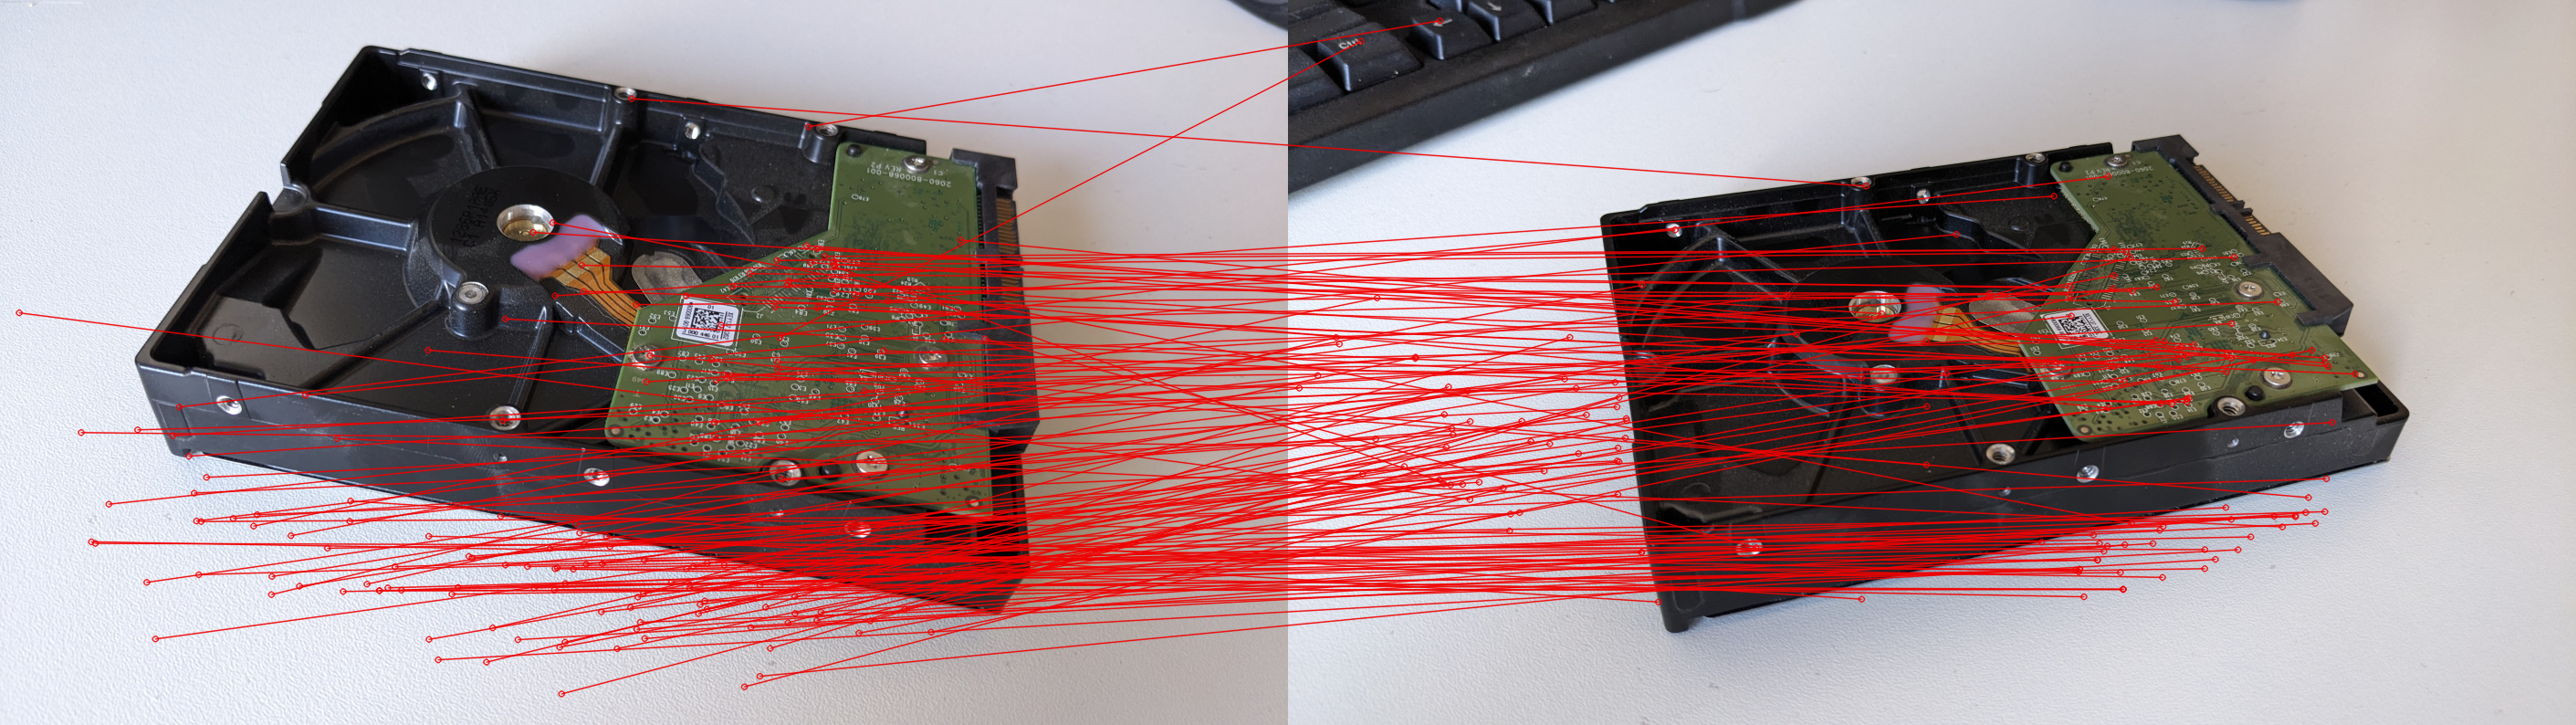
\includegraphics[width=0.88\textwidth]{../figures/a_raw_matches.png}
    \caption{Сирі зіставлення за першим найближчим сусідом до фільтрації Лоу (\texttt{angle4}--\texttt{angle5}, випадкова вибірка $150$ пар із $28624$): численні хаотичні перехресні лінії хибних відповідників}
    \label{fig:raw_matches}
\end{figure}

\begin{figure}[htbp]
    \centering
    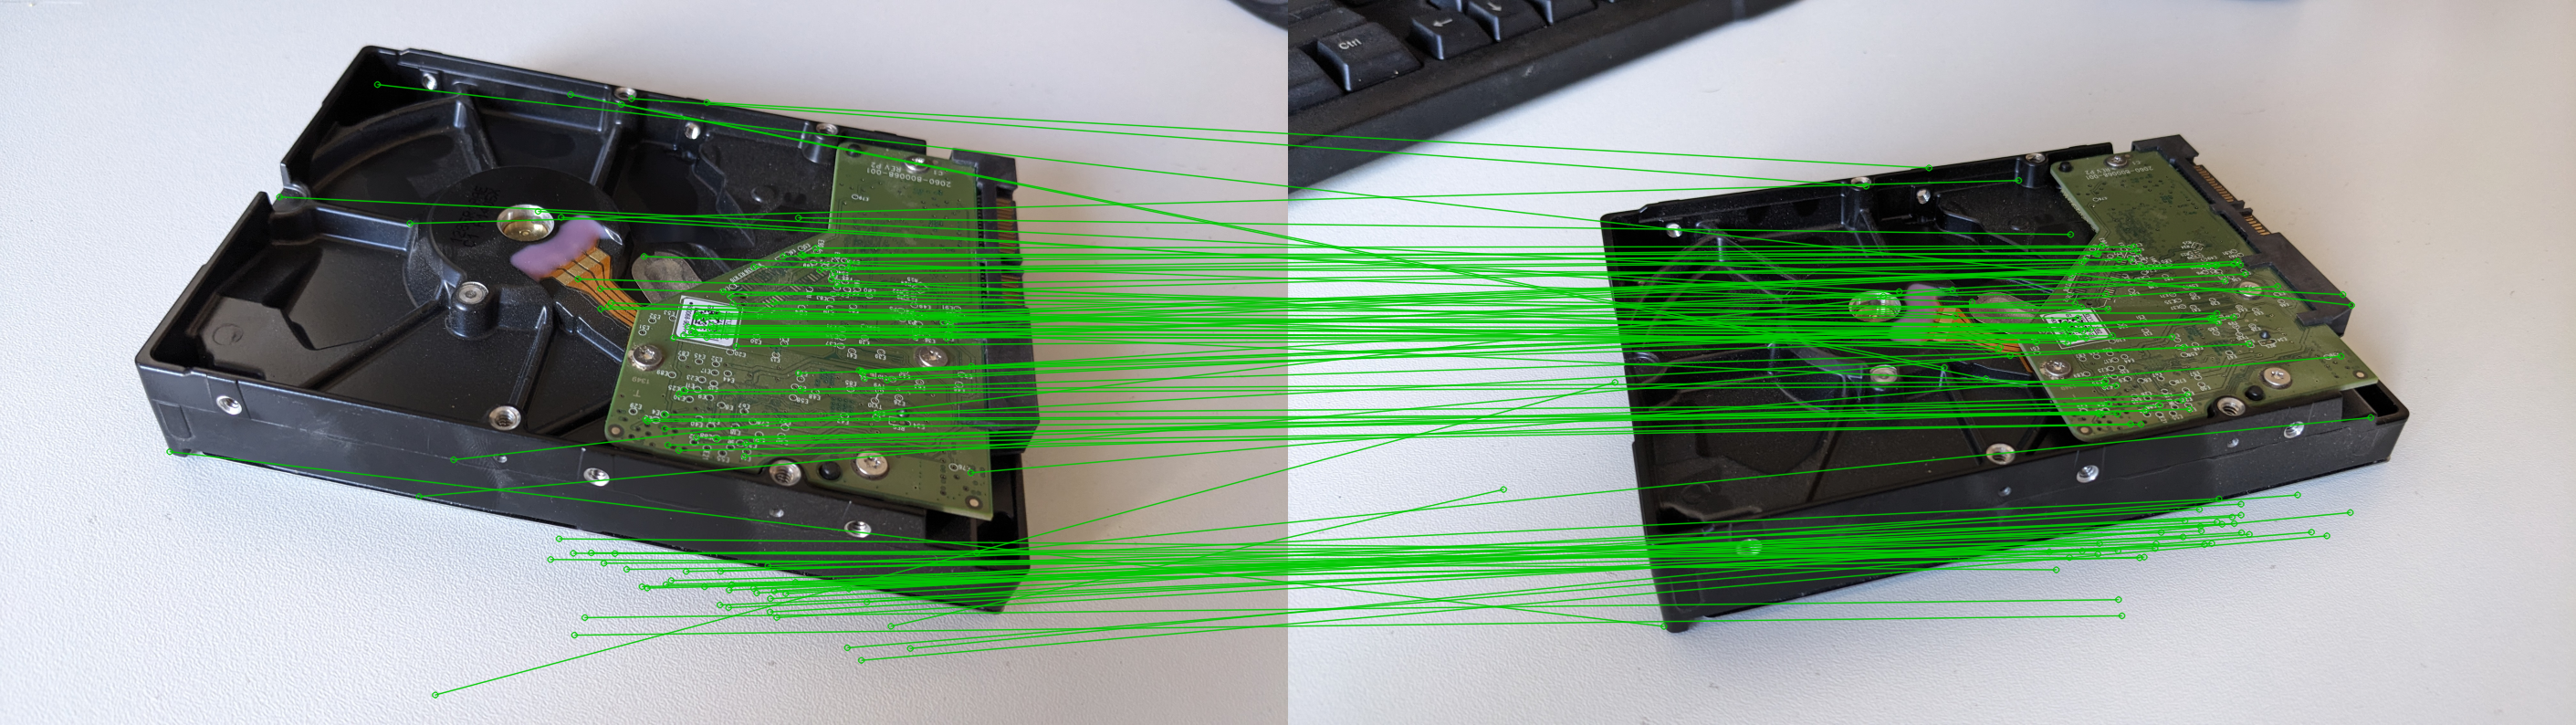
\includegraphics[width=0.88\textwidth]{../figures/a_mutual_matches.png}
    \caption{Зіставлення після фільтрації за критерієм Лоу ($T=0.75$) та взаємної перевірки (\texttt{angle4}--\texttt{angle5}, вибірка $120$ пар із $291$): переважна більшість ліній узгоджена з геометрією сцени}
    \label{fig:mutual_matches}
\end{figure}

\begin{figure}[htbp]
    \centering
    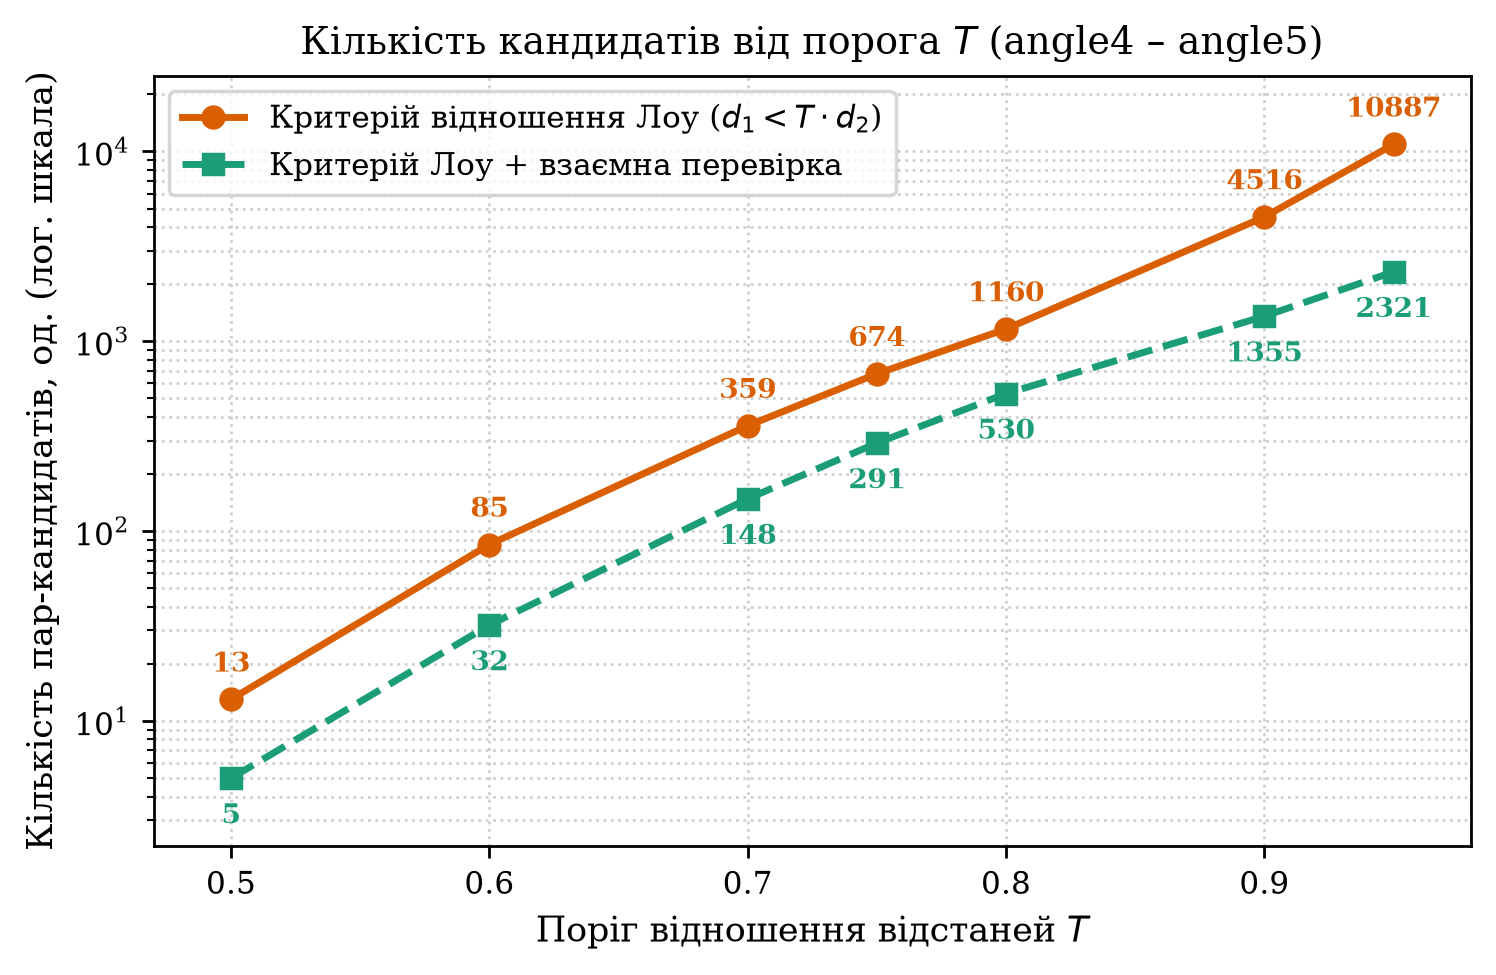
\includegraphics[width=0.76\textwidth]{../figures/a_ratio_curve.png}
    \caption{Залежність кількості відібраних пар-кандидатів від порога відношення відстаней $T$ для пари \texttt{angle4}--\texttt{angle5} (логарифмічна шкала осі ординат)}
    \label{fig:ratio_curve}
\end{figure}

\begin{table}[htbp]
\centering
\caption{Порівняння класичного МНК без відсіву та RANSAC при $T=0.80, \tau=3.0$~пк (Частина B)}
\label{tab:ols_vs_ransac}
\scriptsize
\setlength{\tabcolsep}{3.5pt}
\begin{tabular}{cccccccc}
\toprule
Пара & Кандидати & Inliers & Outliers & МНК (усі) & МНК (inliers) & RANSAC mean & RANSAC med \\
\midrule
\directlua{tab_ols_vs_ransac()}
\bottomrule
\end{tabular}
\end{table}

\begin{figure}[htbp]
    \centering
    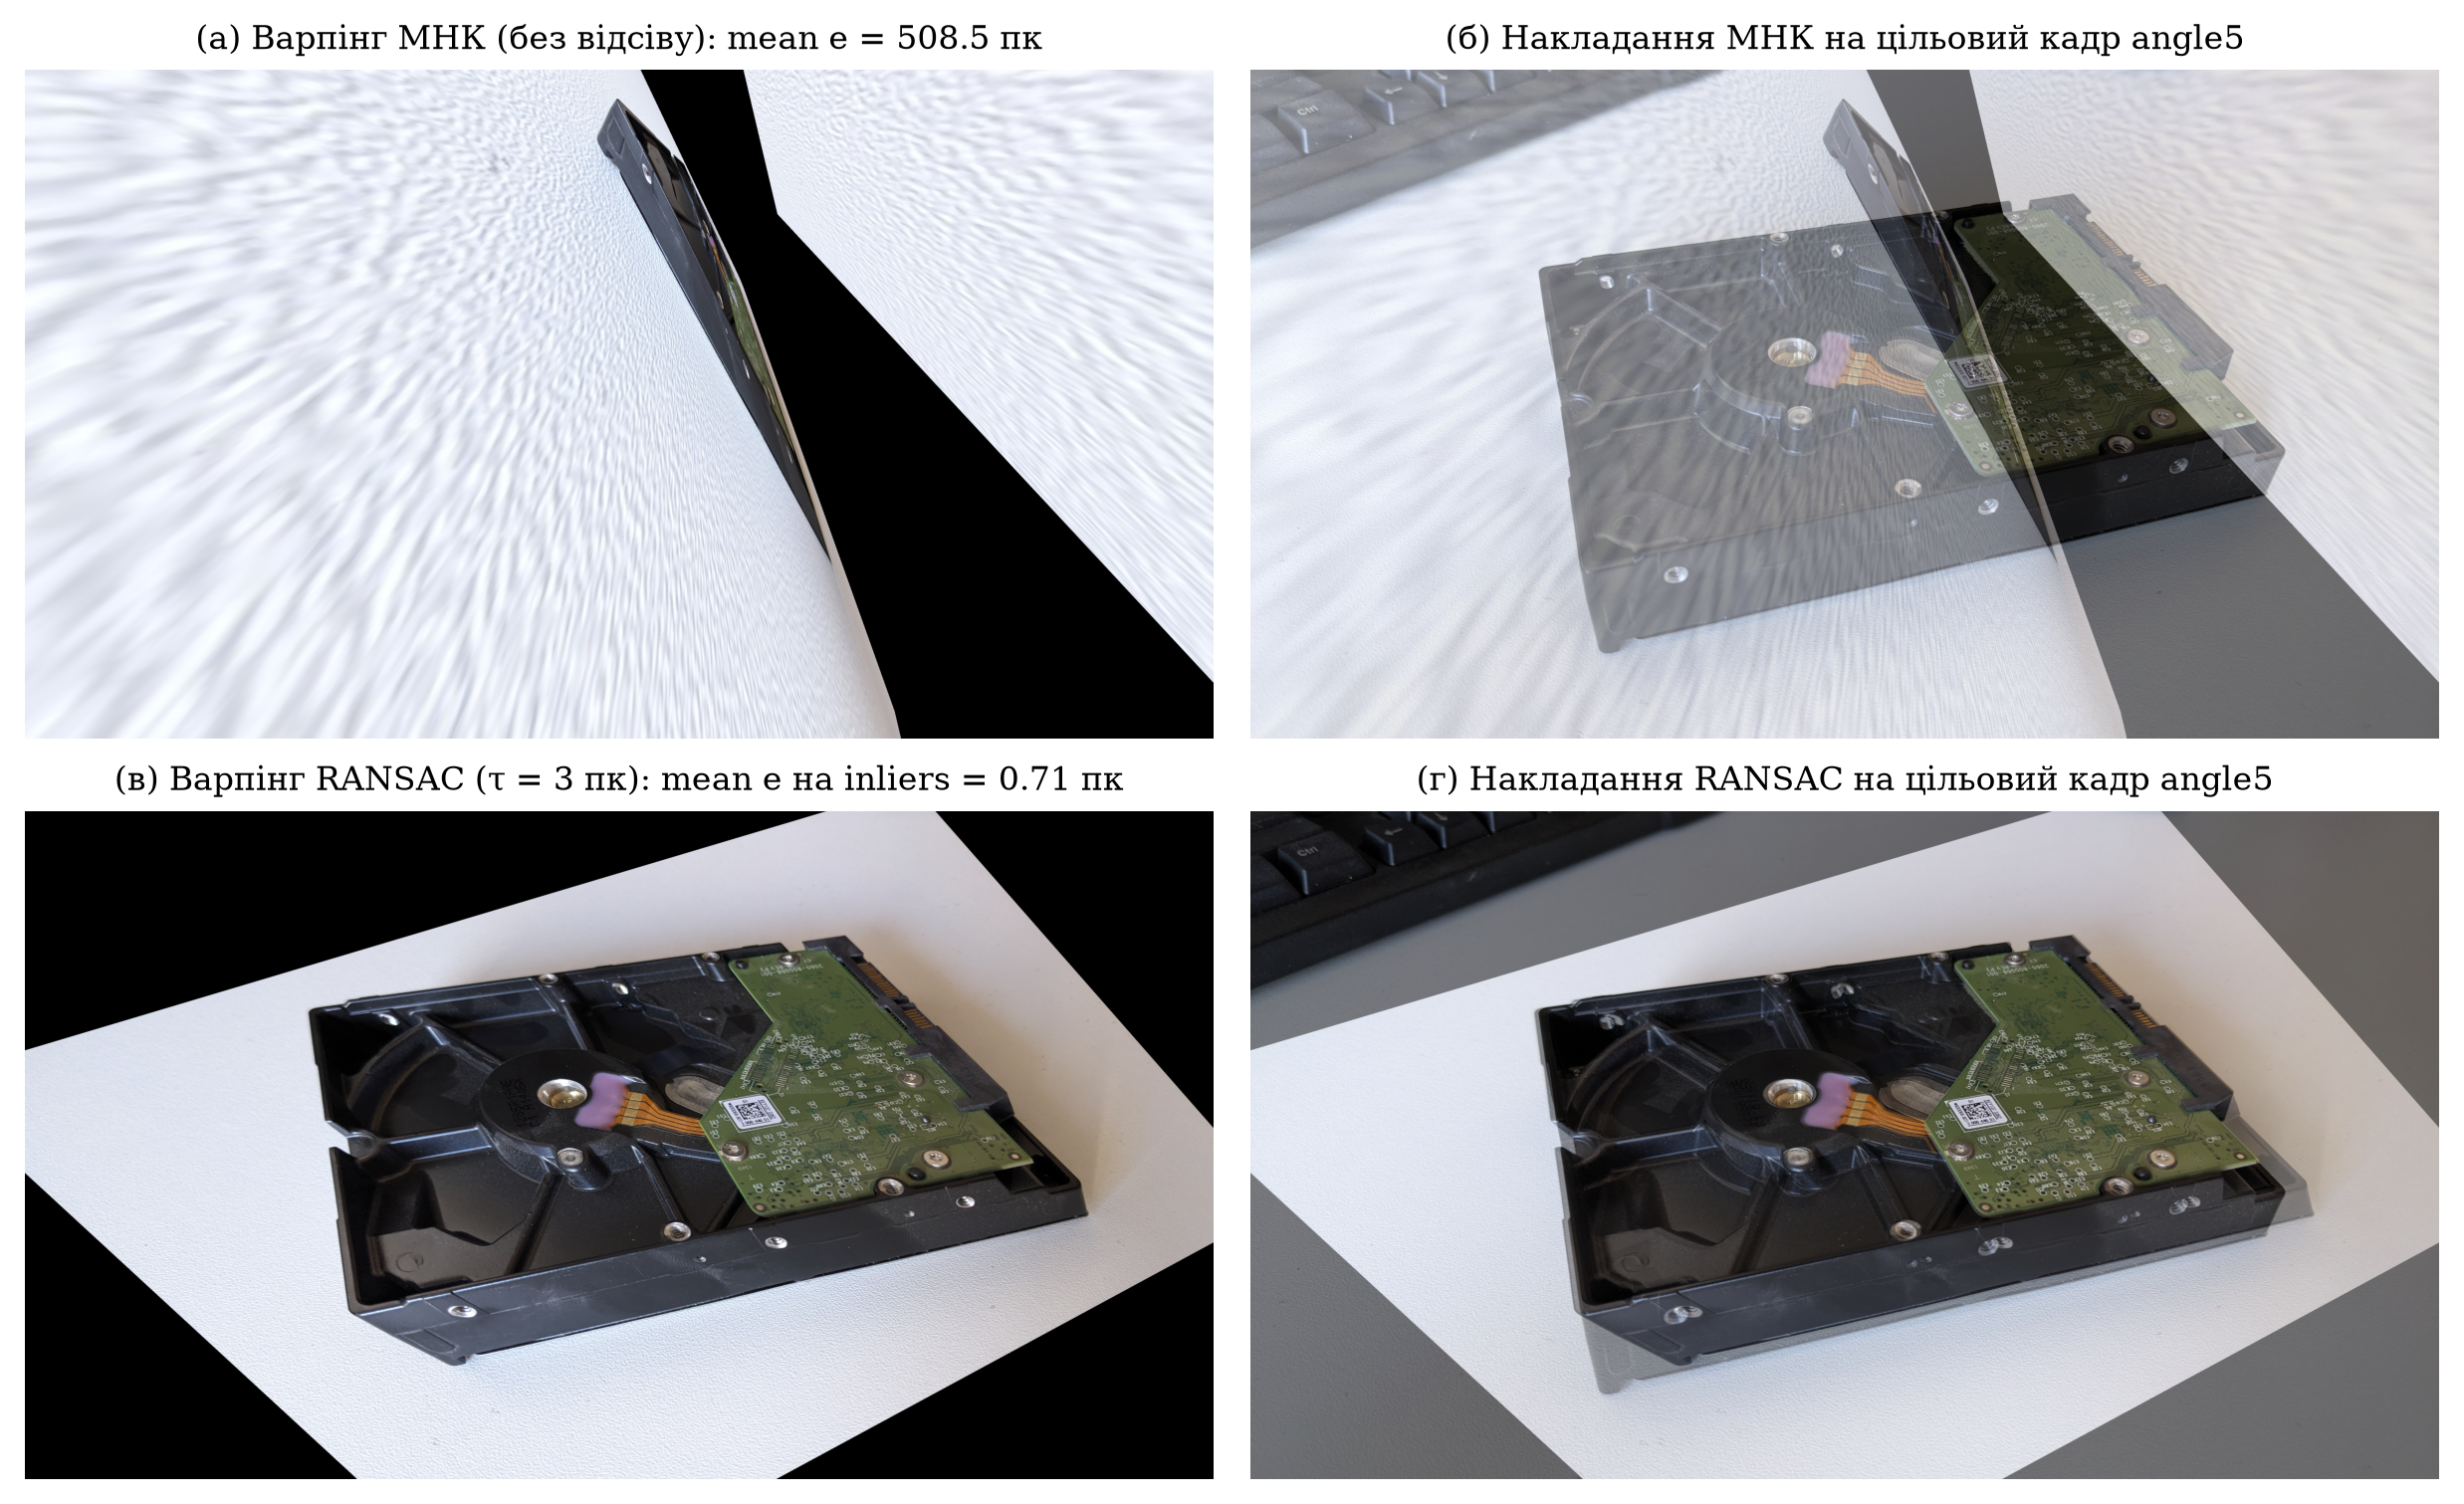
\includegraphics[width=0.96\textwidth]{../figures/b_ols_vs_ransac_panel.png}
    \caption{Порівняння переносу кадру \texttt{angle4} у координати \texttt{angle5}: (а) варпінг за $H_{\text{OLS}}$ ($e_{\text{mean}} = 508.5$~пк); (б) накладання МНК на \texttt{angle5}; (в) варпінг за $H_{\text{RANSAC}}$ ($\tau=3$~пк, $e_{\text{mean}} = 0.71$~пк на inliers); (г) накладання RANSAC на \texttt{angle5}}
    \label{fig:ols_panel}
\end{figure}

\begin{figure}[htbp]
    \centering
    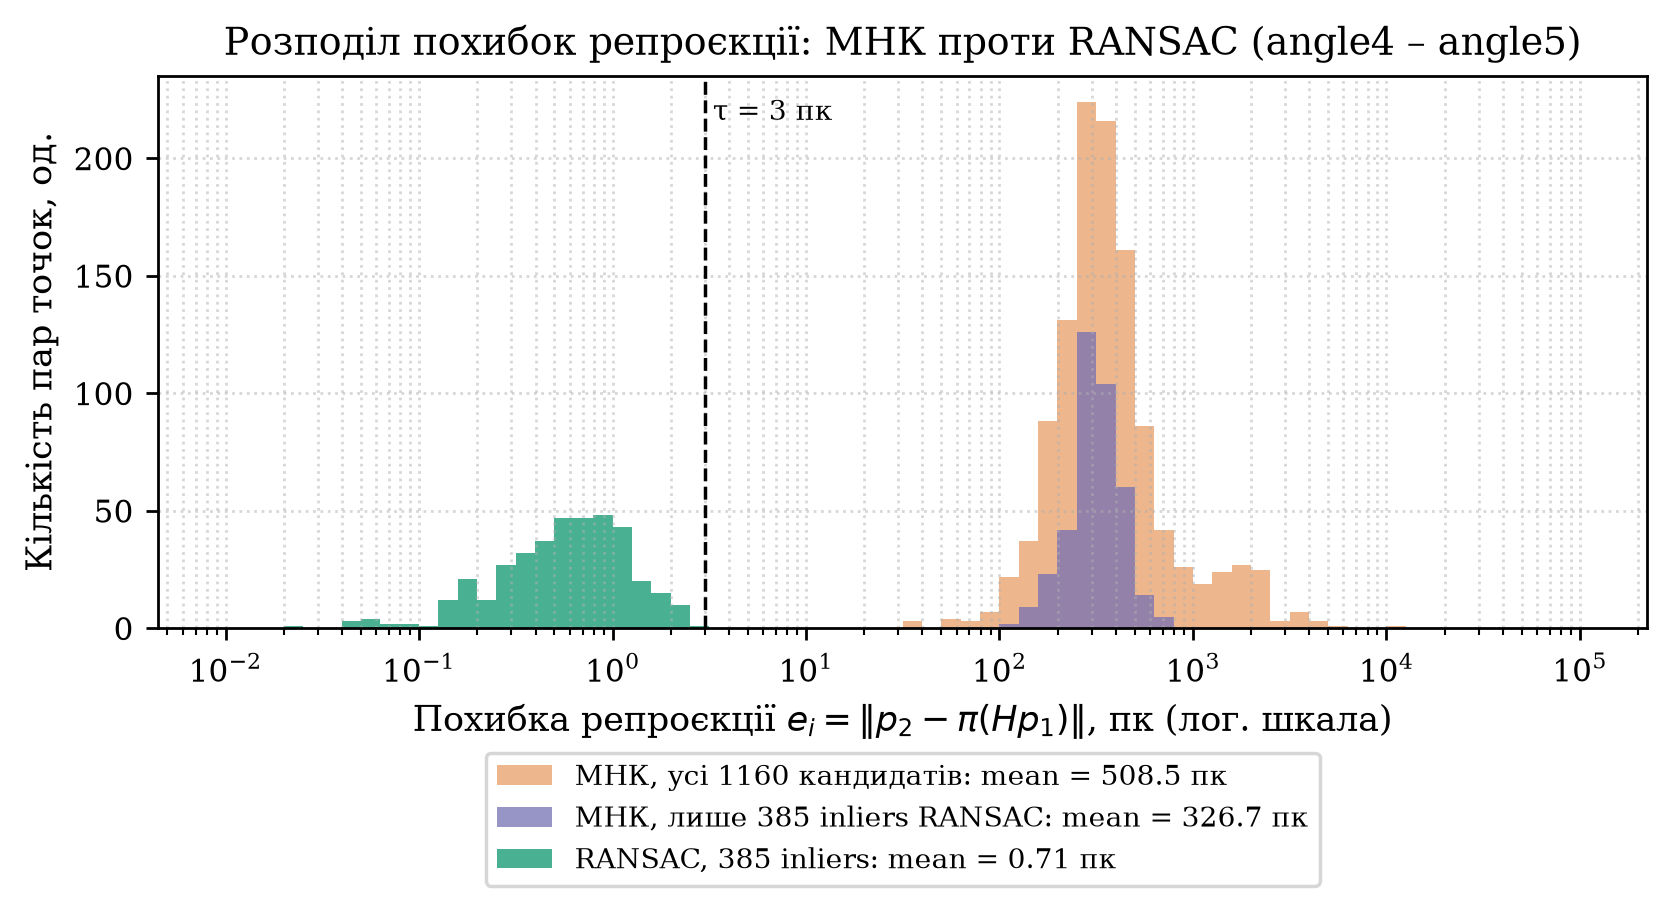
\includegraphics[width=0.80\textwidth]{../figures/b_reprojection_hist.png}
    \caption{Гістограма розподілу похибок репроєкції (лог. шкала): МНК на всіх $1160$ кандидатах, МНК на $385$ істинних inliers та RANSAC на тих самих $385$ inliers}
    \label{fig:reproj_hist}
\end{figure}

\begin{table}[htbp]
\centering
\caption{Порівняння стратегій вибору кількості ітерацій RANSAC за $30$ запусками на парі \texttt{angle4}--\texttt{angle5} (Частина C, у дужках -- теоретична ймовірність успіху за формулою~\eqref{eq:ransac_iters})}
\label{tab:ransac_iterations}
\footnotesize
\setlength{\tabcolsep}{4.5pt}
\begin{tabular}{lccccc}
\toprule
Стратегія ітераційного бюджету & Ітерацій & Inliers (mean $\pm \sigma$) & Успіх (теор.) & Похибка & Час \\
\midrule
\directlua{tab_ransac_iterations()}
\bottomrule
\end{tabular}
\end{table}

\begin{table}[htbp]
\centering
\caption{Звірка власної реалізації RANSAC із бібліотечною функцією \texttt{cv2.findHomography} ($\tau = 3.0$~пк; спільних inliers: $378$, IoU $= 97.9\%$, середнє розходження проєкцій на спільних точках $0.36$~пк)}
\label{tab:ransac_comparison}
\footnotesize
\begin{tabular}{lcccc}
\toprule
Реалізація & Inliers, од. & Похибка (власні inliers) & Похибка (спільні $378$ точок) & Час, мс \\
\midrule
\directlua{tab_ransac_comparison()}
\bottomrule
\end{tabular}
\end{table}

\begin{table}[htbp]
\centering
\caption{Залежність об'єму консенсусу та похибки репроєкції від порога узгодженості $\tau$ за $10$ запусками (Частина C)}
\label{tab:ransac_threshold}
\footnotesize
\begin{tabular}{ccccc}
\toprule
Поріг $\tau$ & Inliers (власний, mean $\pm \sigma$) & Частка від кандидатів & Похибка (mean $\pm \sigma$) & Inliers (OpenCV) \\
\midrule
\directlua{tab_ransac_threshold()}
\bottomrule
\end{tabular}
\end{table}

\begin{figure}[htbp]
    \centering
    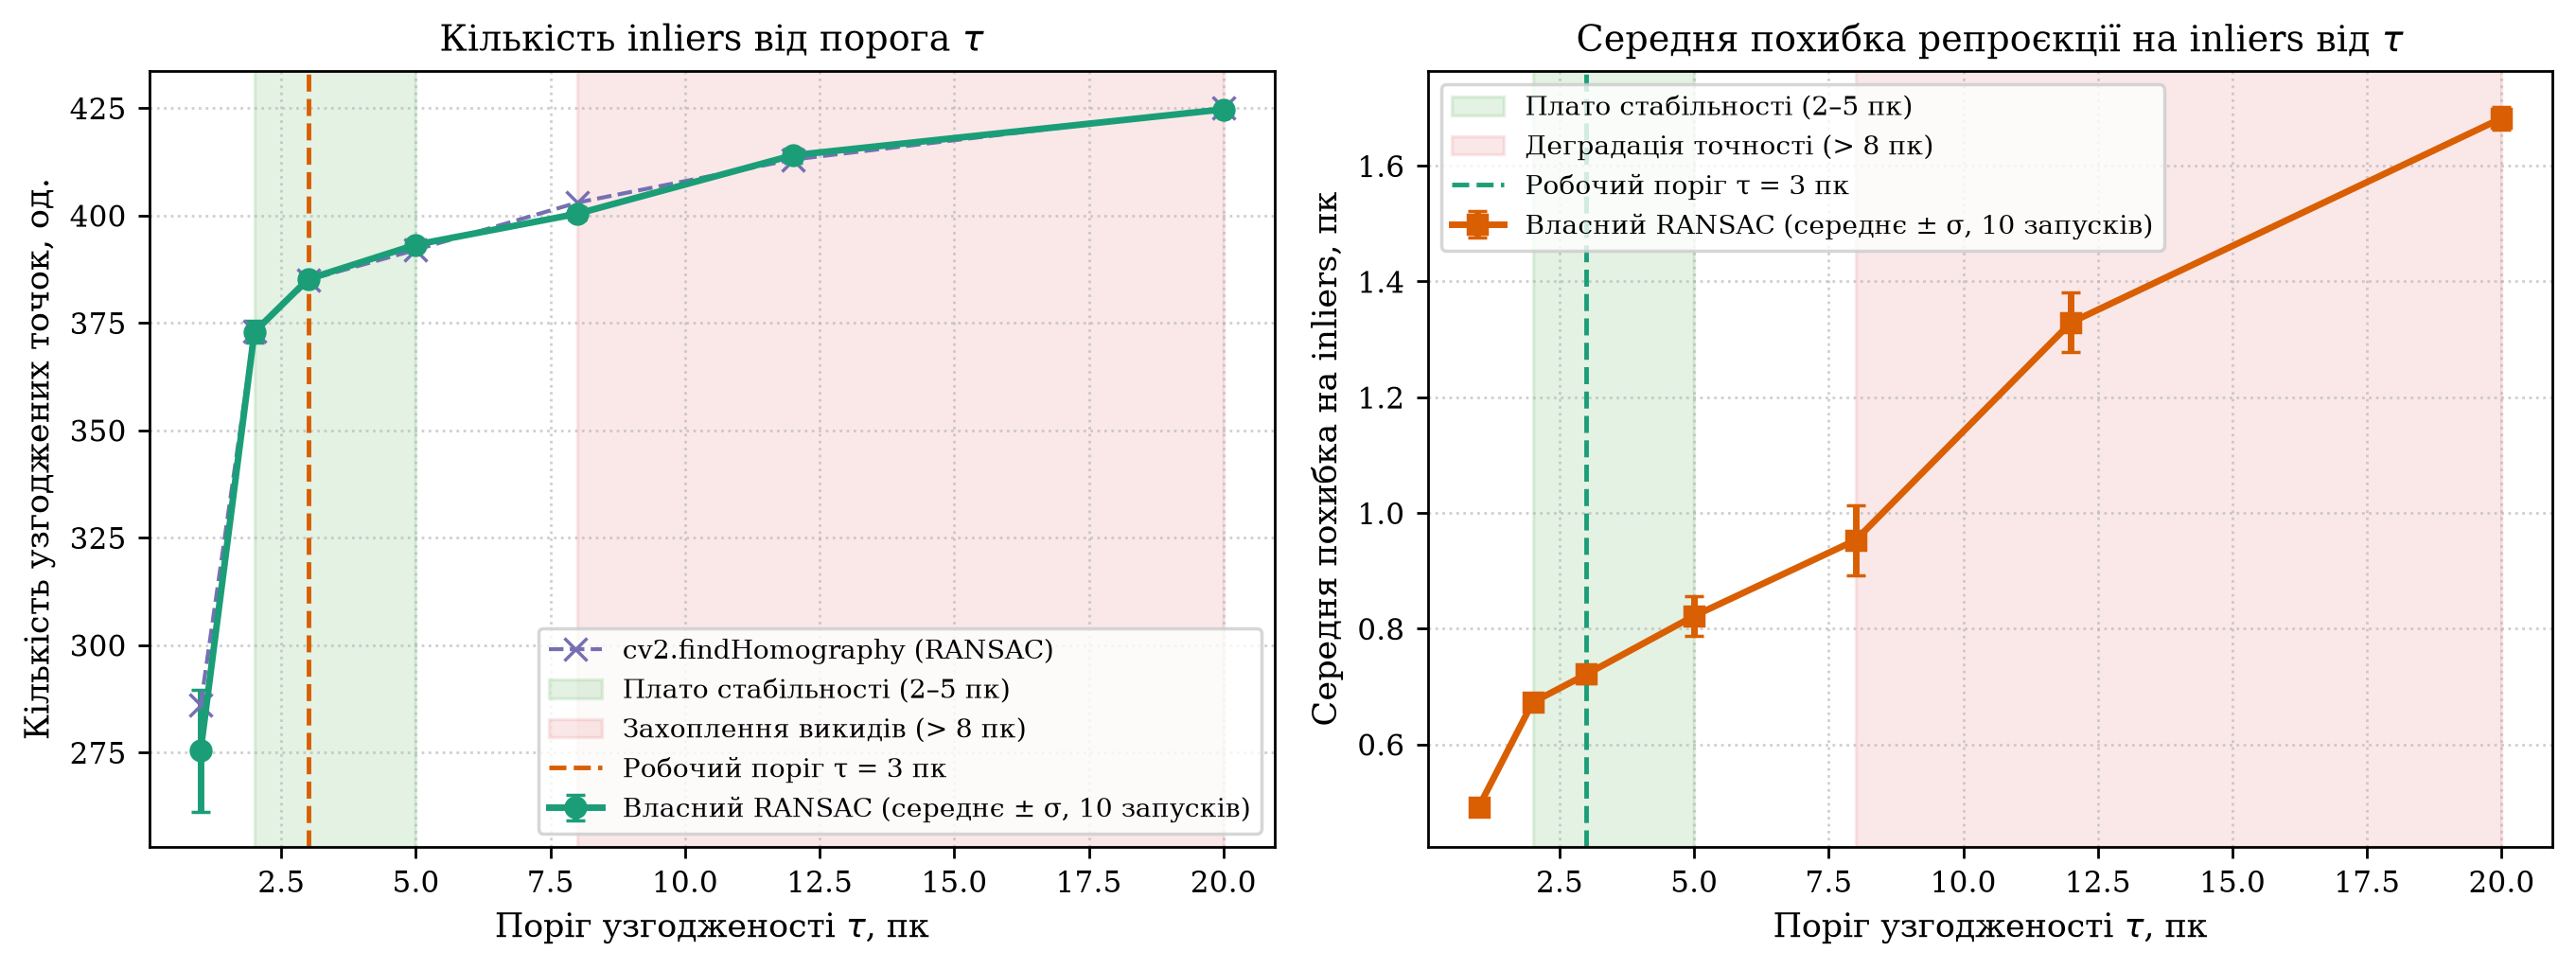
\includegraphics[width=0.98\textwidth]{../figures/c_threshold_analysis.png}
    \caption{Дослідження порога $\tau$ (середнє $\pm \sigma$ за $10$ запусками): (ліворуч) кількість inliers порівняно з \texttt{cv2.findHomography}; (праворуч) середня похибка репроєкції на inliers}
    \label{fig:threshold_curves}
\end{figure}

\begin{figure}[htbp]
    \centering
    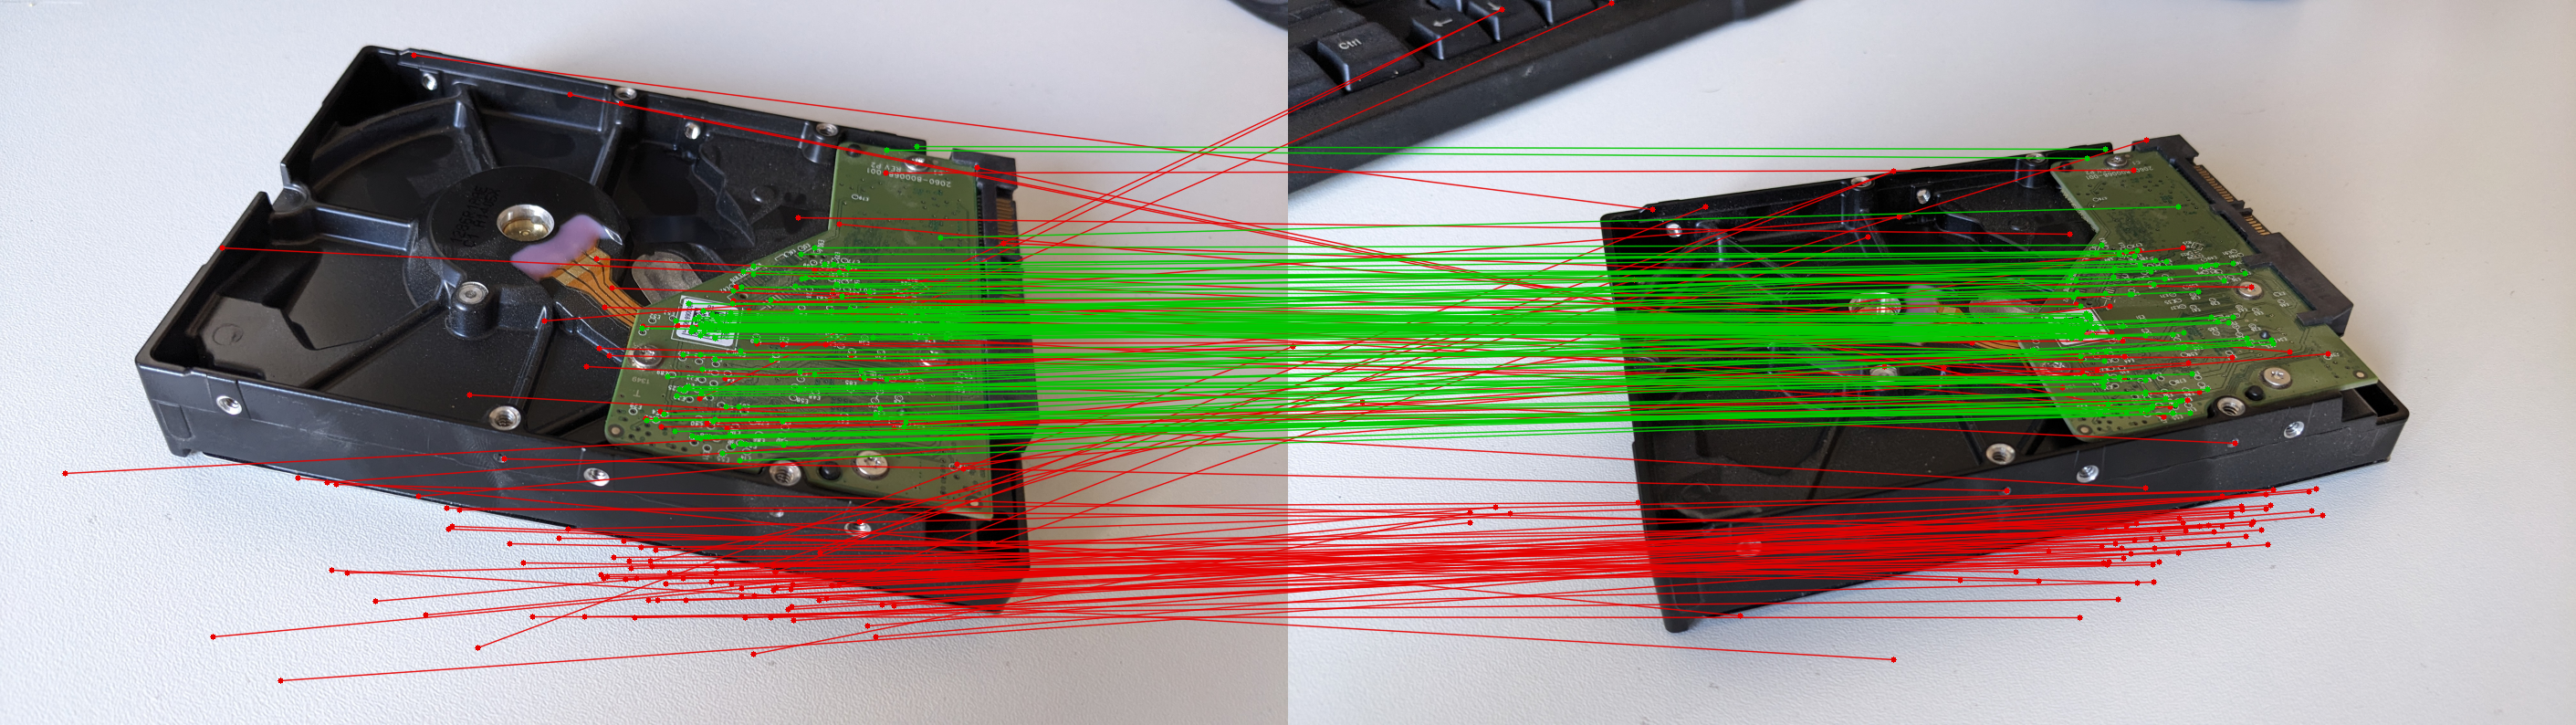
\includegraphics[width=0.92\textwidth]{../figures/c_inliers_outliers.png}
    \caption{Візуалізація класифікації RANSAC ($\tau=3.0$~пк) для пари \texttt{angle4}--\texttt{angle5}: зелені лінії -- узгоджені зіставлення (вибірка $120$ із $379$ inliers, $e_{\text{mean}} = 0.78$~пк); червоні лінії -- відкинуті викиди ($120$ із $781$ outliers)}
    \label{fig:inliers_outliers}
\end{figure}

\begin{table}[htbp]
\centering
\caption{Об'єктивна оцінка геометричної якості сусідніх пар панорамної серії \texttt{corner\_7}--\texttt{corner\_3} (Частина D, інтегральна середня похибка на всіх $4042$ inliers становить $0.73$~пк)}
\label{tab:panorama_quality}
\footnotesize
\begin{tabular}{ccccccc}
\toprule
Сусідня пара & Кандидати & Inliers & Частка inliers & $e_{\text{mean}}$ & $e_{\text{std}}$ & $e_{\text{max}}$ \\
\midrule
\directlua{tab_panorama_quality()}
\bottomrule
\end{tabular}
\end{table}

\begin{figure}[htbp]
    \centering
    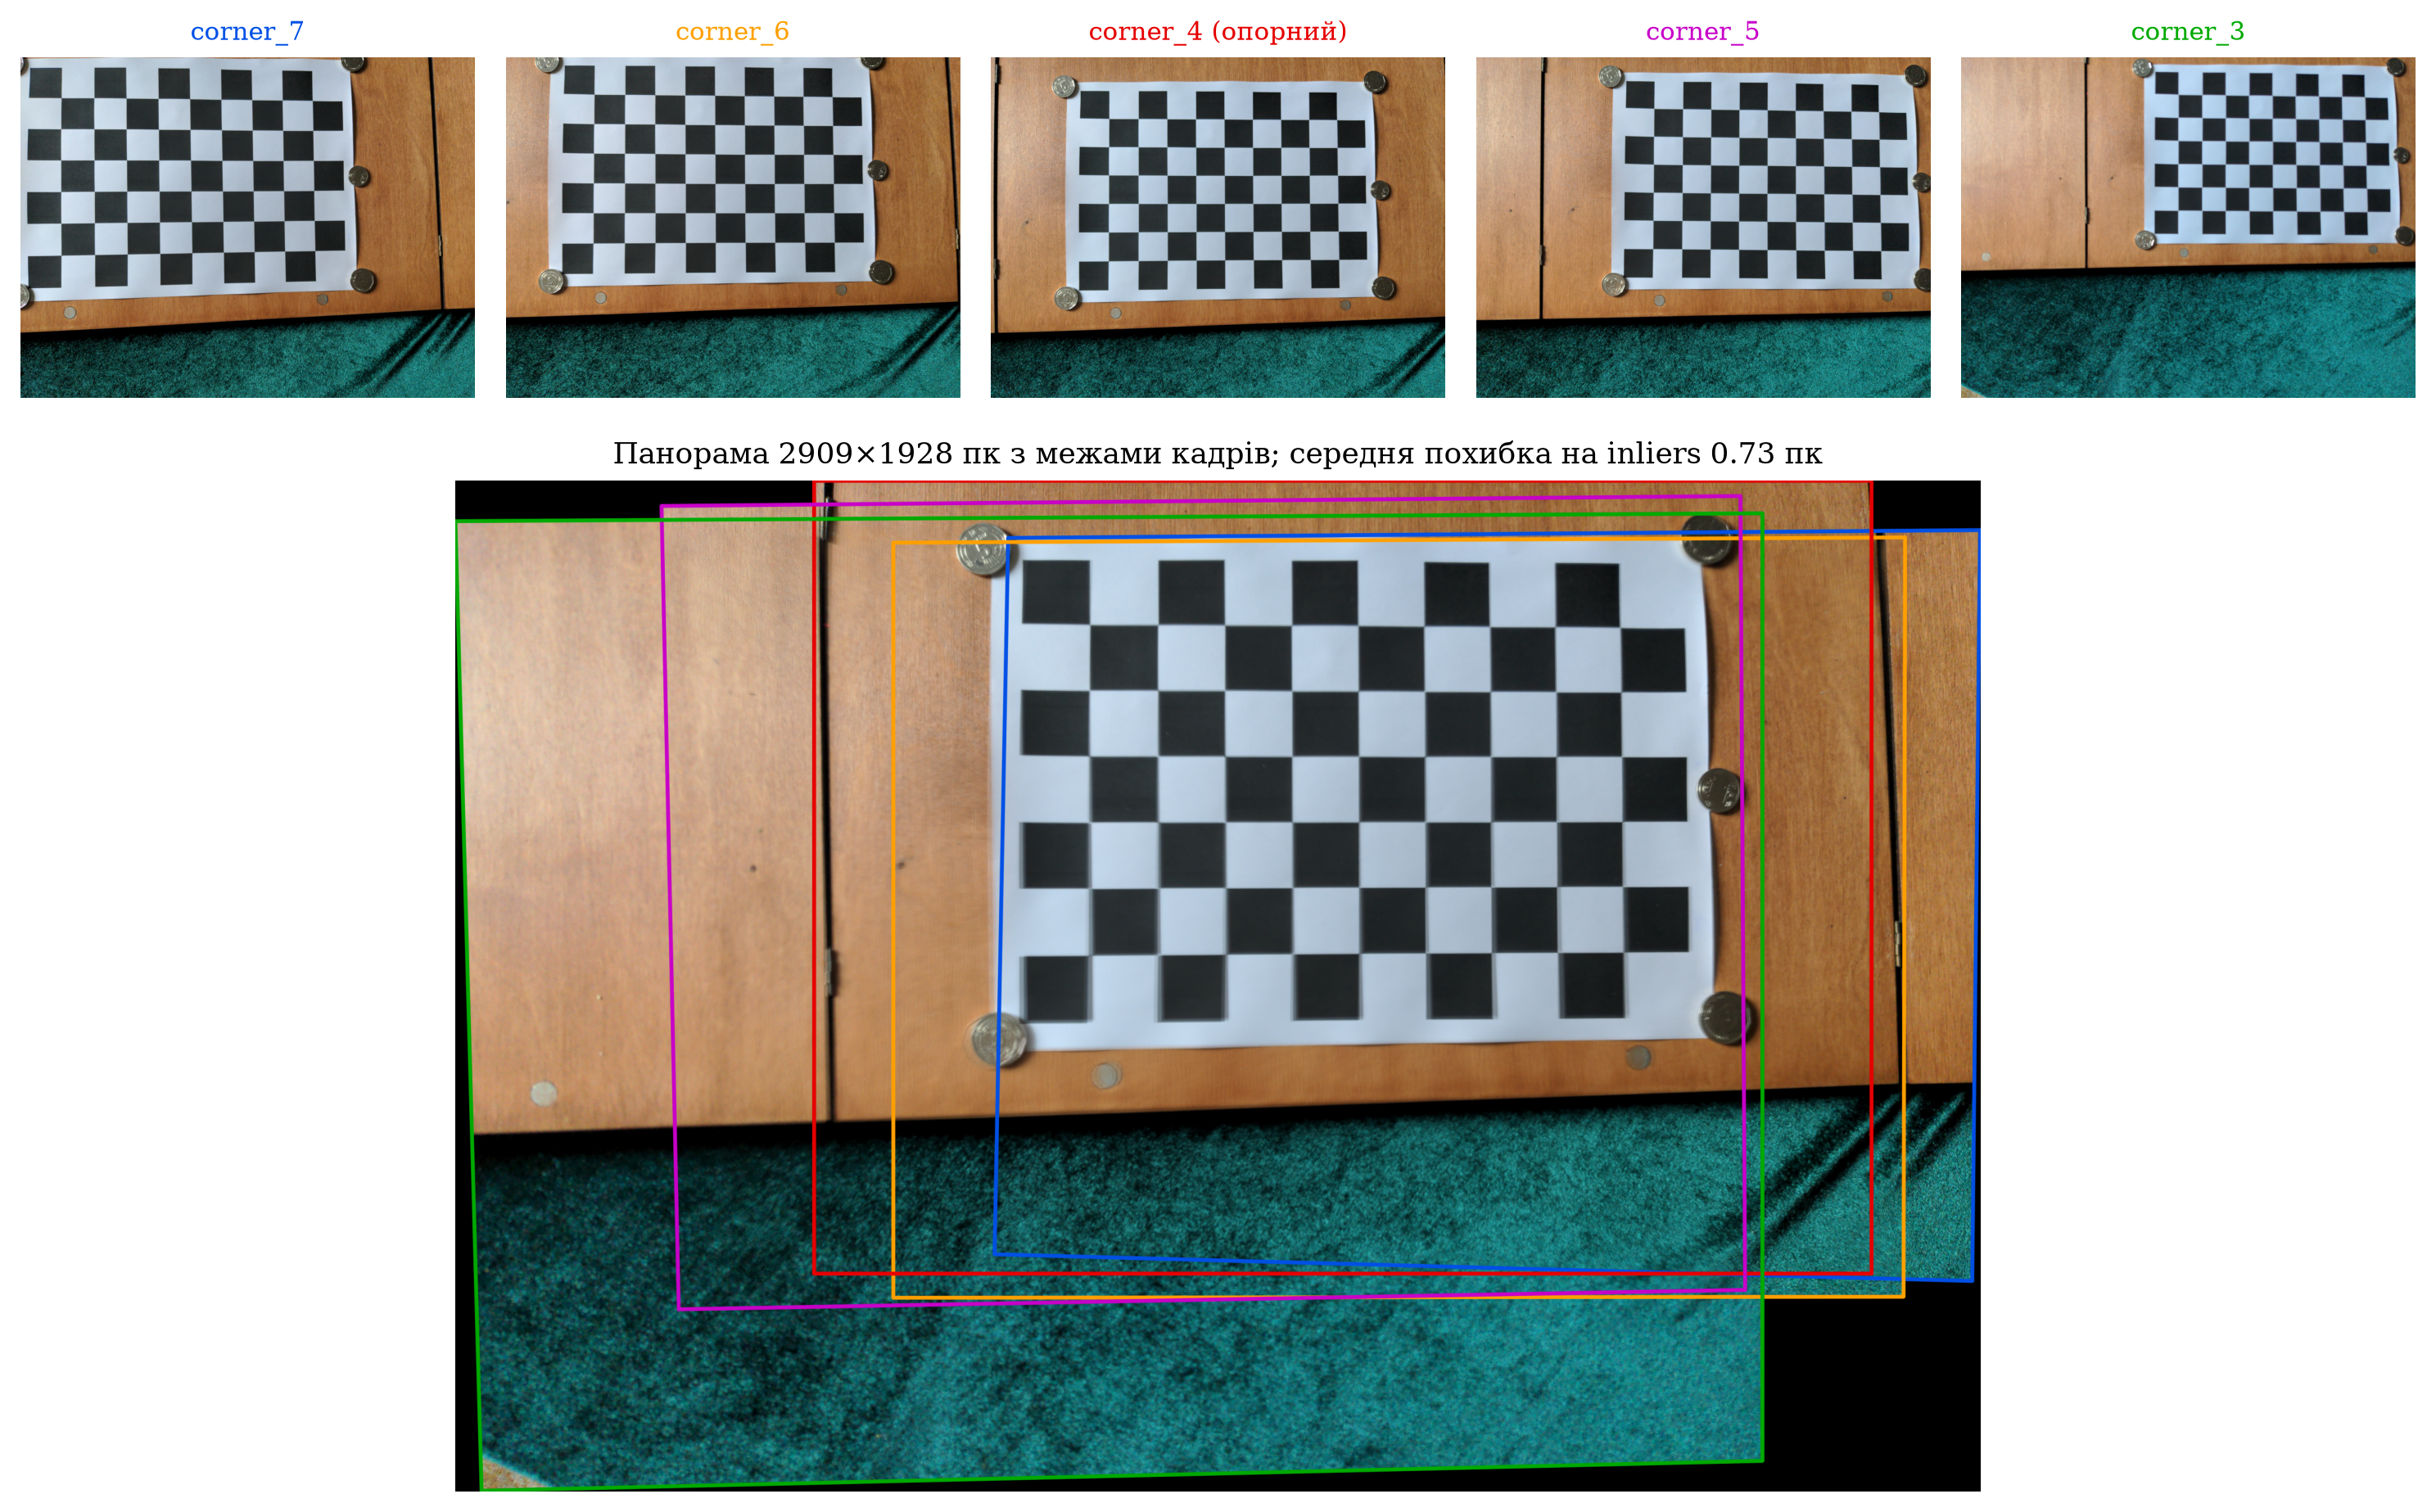
\includegraphics[width=0.98\textwidth]{../figures/d_panorama_overview.png}
    \caption{Побудова панорами плоскої сцени з 5 кадрів (\texttt{lab02/data/corners/}): (вгорі) вхідні кадри \texttt{corner\_7}, \texttt{corner\_6}, \texttt{corner\_4} (опорний), \texttt{corner\_5}, \texttt{corner\_3}; (внизу) полотно $2909 \times 1928$~пк із кольоровими рамками проєкцій кадрів}
    \label{fig:panorama_overview}
\end{figure}

\begin{figure}[htbp]
    \centering
    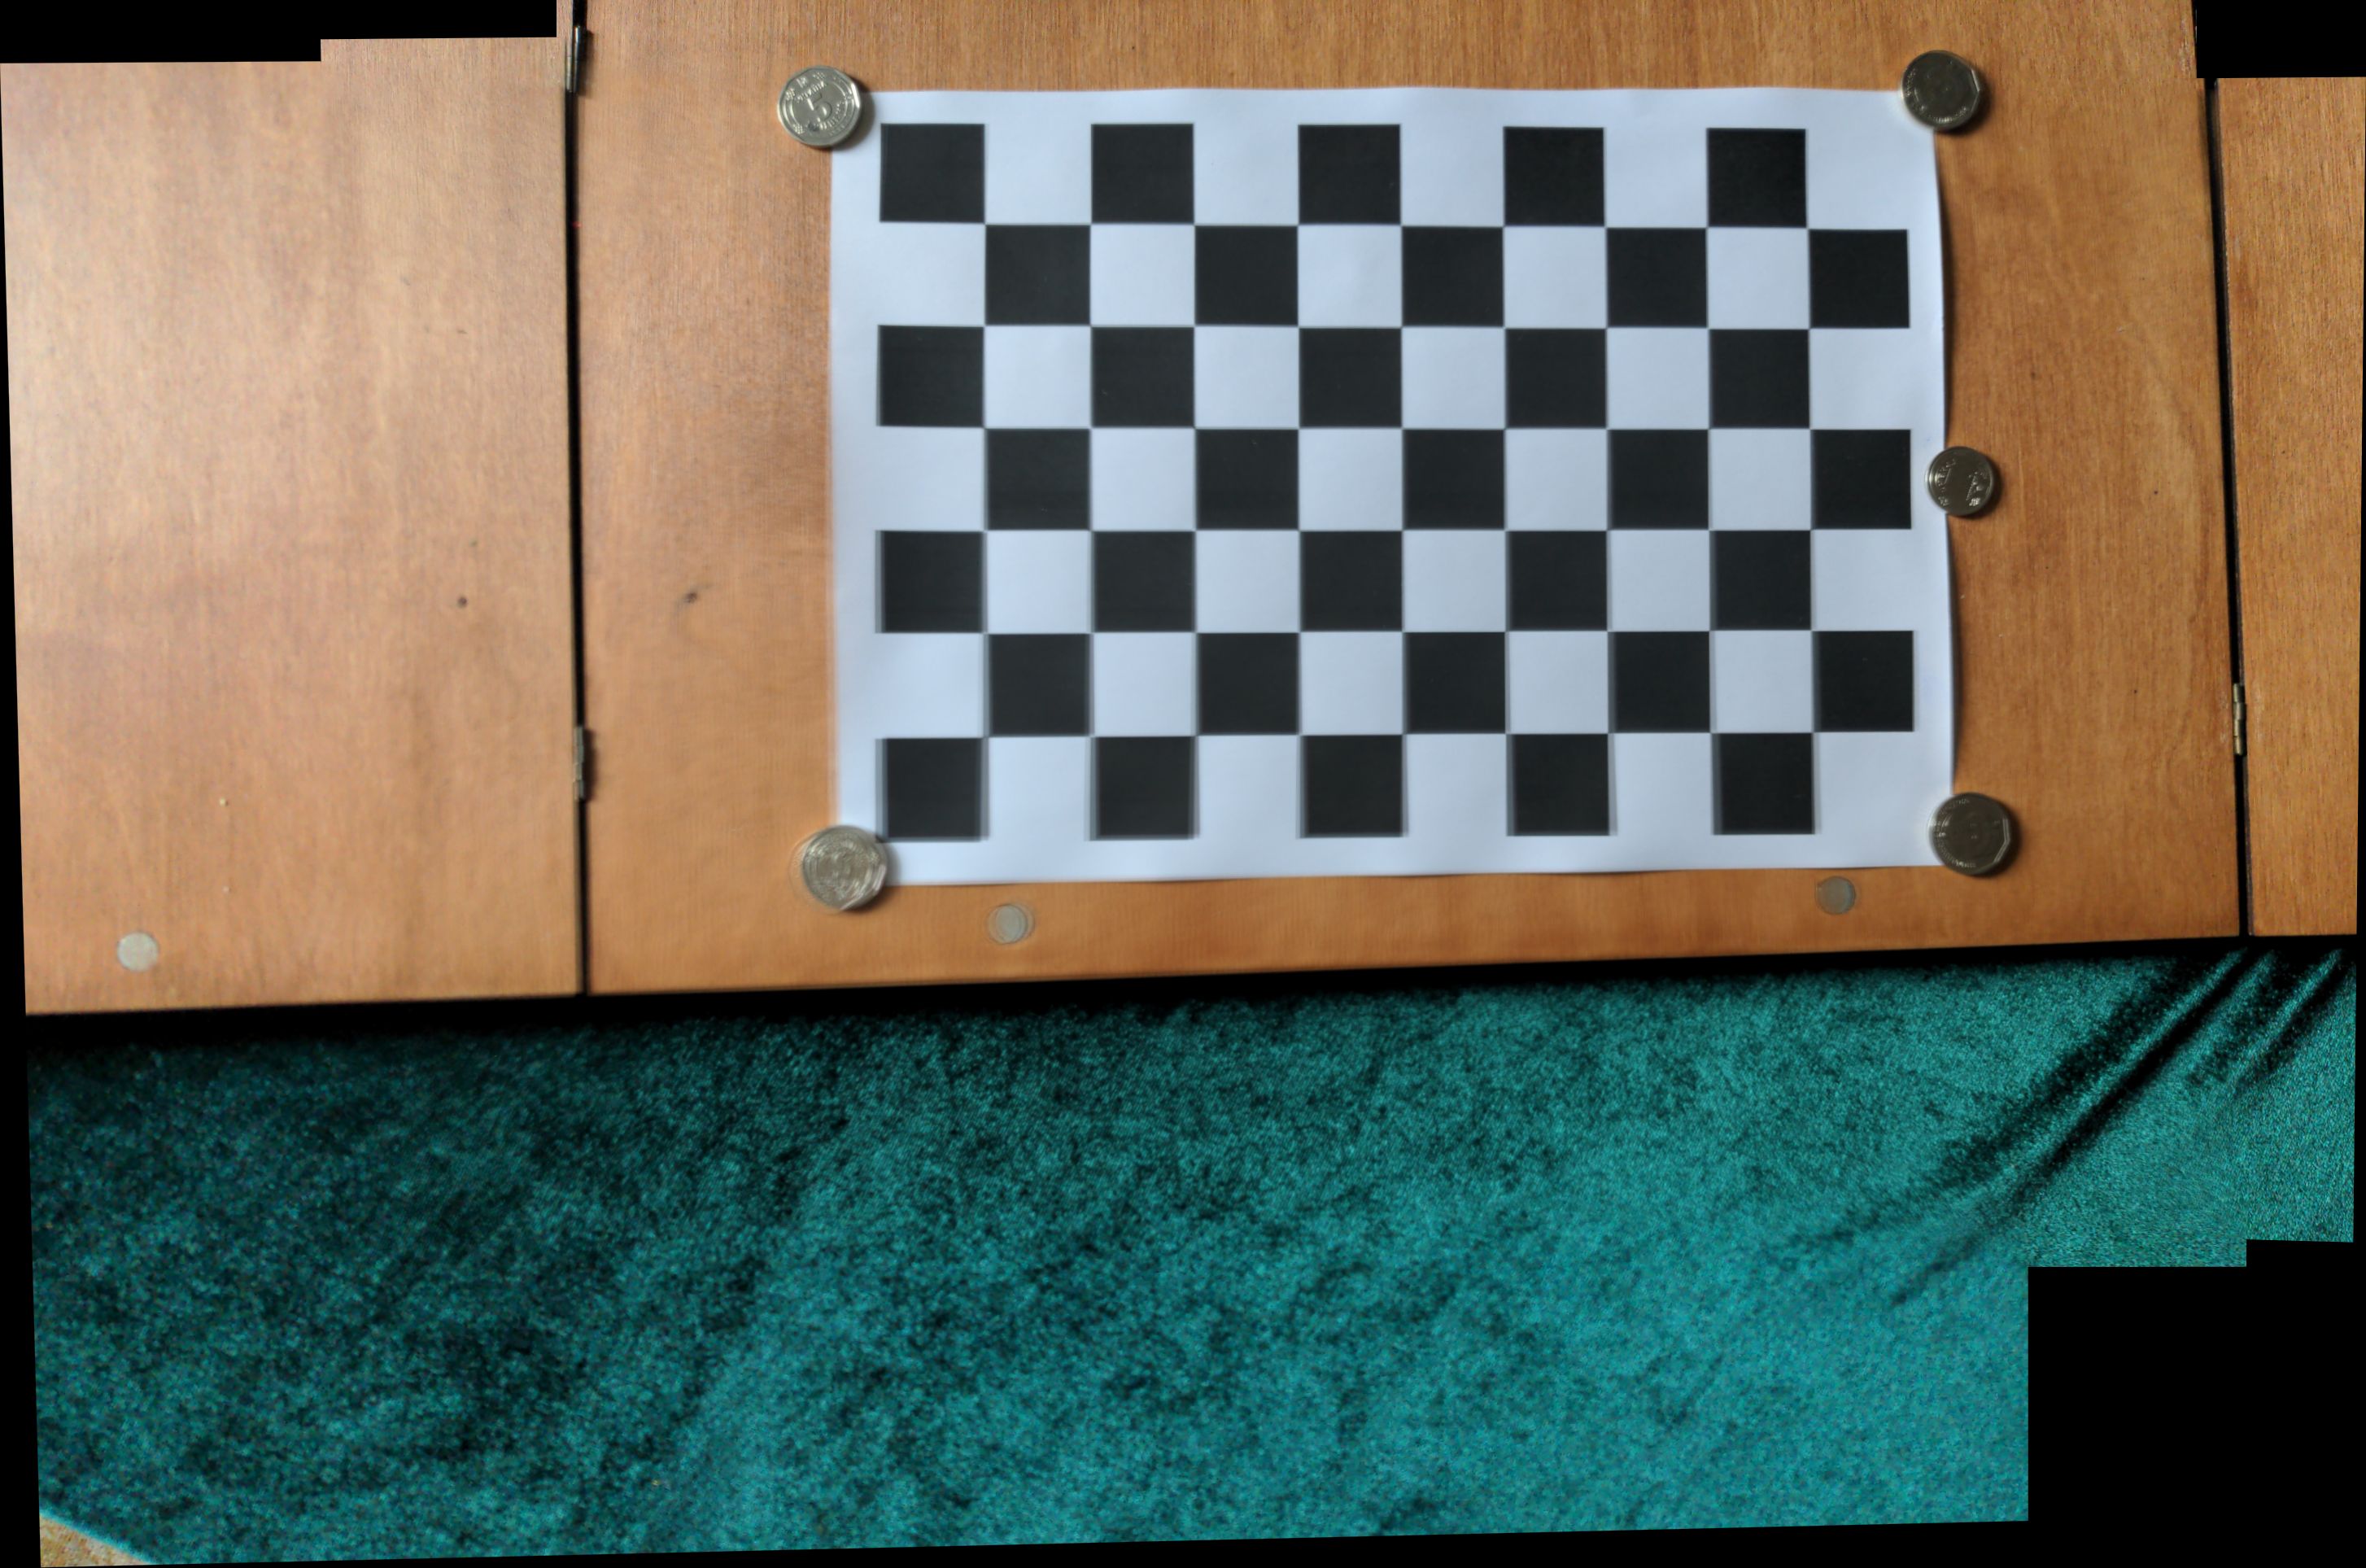
\includegraphics[width=0.94\textwidth]{../figures/d_panorama.png}
    \caption{Фінальна безшовна панорама з 5 кадрів ($2908 \times 1927$~пк, лінійне вагове блендування \texttt{distanceTransform}, інтегральна середня похибка репроєкції $0.73$~пк)}
    \label{fig:panorama_final}
\end{figure}

\begin{table}[htbp]
\centering
\caption{Дослідження перекриття кадрів та геометричної правдоподібності гомографії (Частина E; перекриття подано як покриття цільового кадру / видима частка першого кадру)}
\label{tab:overlap_failure}
\scriptsize
\setlength{\tabcolsep}{2.2pt}
\begin{tabular}{lp{1.90cm}ccccp{1.60cm}}
\toprule
Пара & Характеристика & Канд. & Inliers & Перекриття & $e_{\text{mean}}$ & Статус \\
\midrule
\directlua{tab_overlap_failure()}
\bottomrule
\end{tabular}
\end{table}

\begin{table}[htbp]
\centering
\caption{Кількісний прояв просторового паралаксу при зшиванні 3D-серії жорсткого диска \texttt{angle2}--\texttt{angle6} (Частина E): похибка на площині плати проти медіанного відхилення взаємних збігів поза платою}
\label{tab:parallax_pairs}
\footnotesize
\begin{tabular}{ccccc}
\toprule
Сусідня пара & Взаємні кандидати & Inliers на платі & $e_{\text{mean}}$ (плата) & Медіана $e$ (поза платою) \\
\midrule
\directlua{tab_parallax_pairs()}
\bottomrule
\end{tabular}
\end{table}

\begin{figure}[htbp]
    \centering
    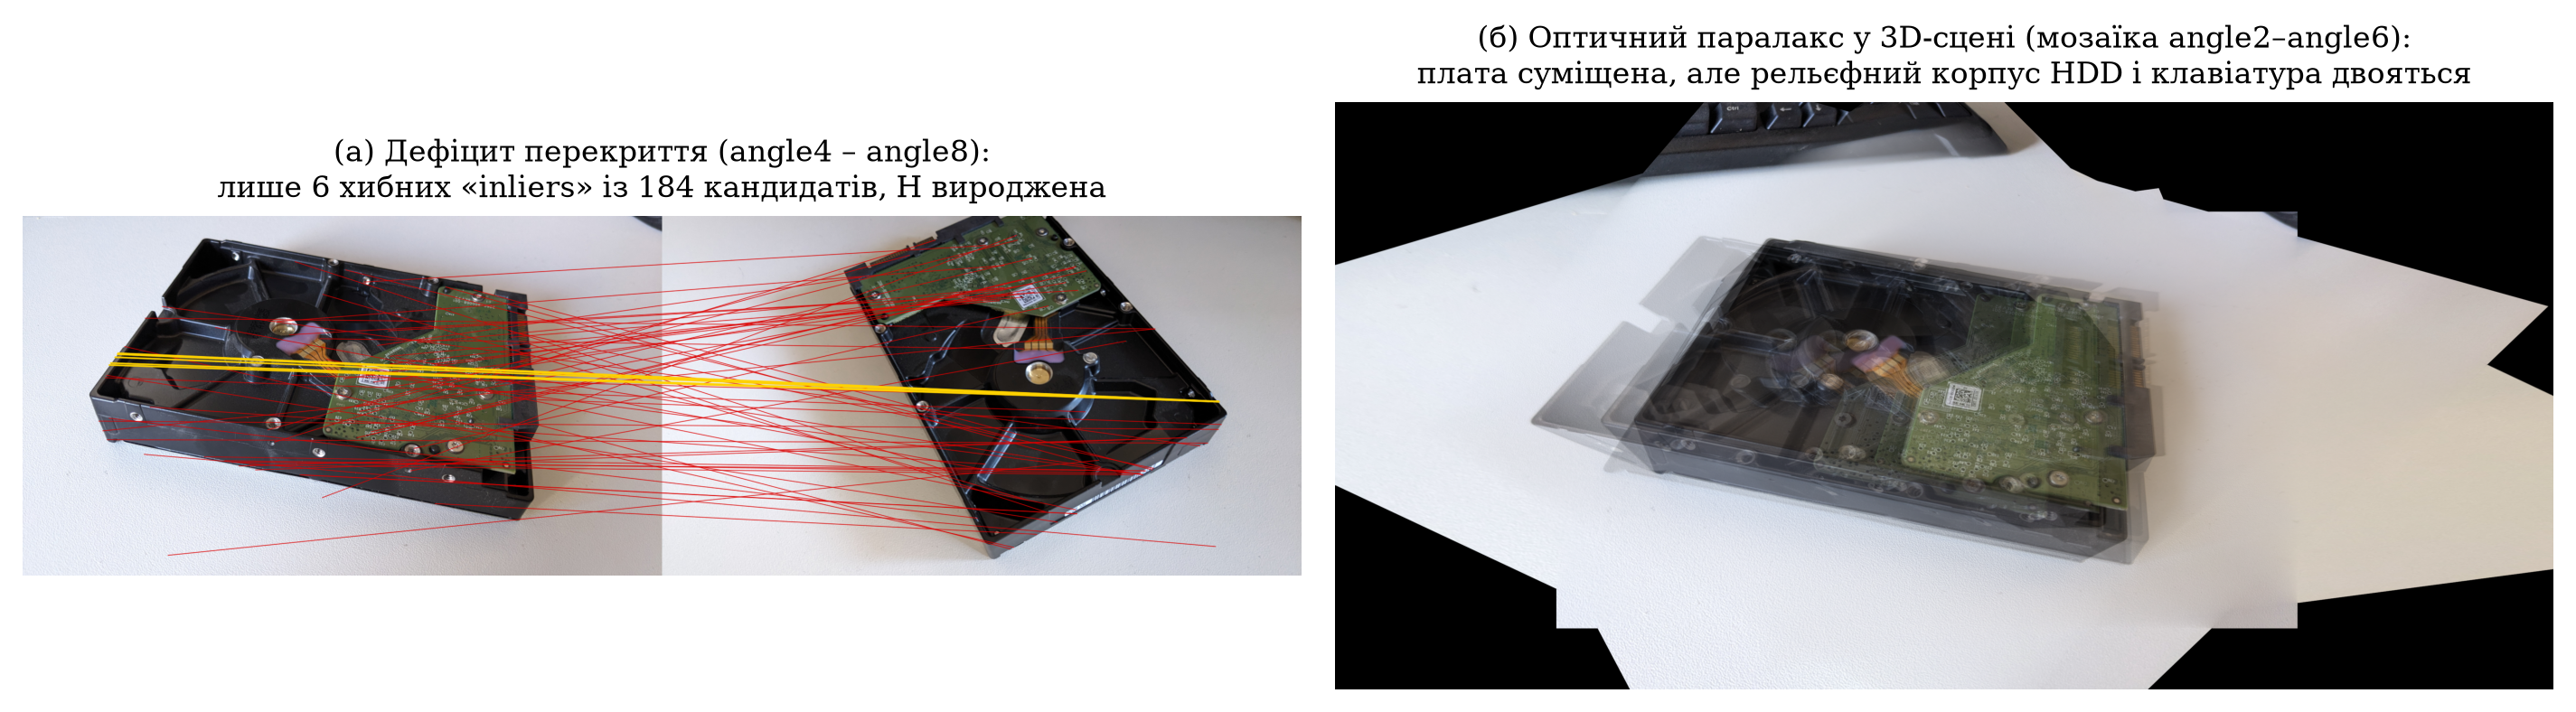
\includegraphics[width=0.98\textwidth]{../figures/e_failure_cases.png}
    \caption{Типові випадки відмови гомографічного зшивання: (а) дефіцит перекриття на парі \texttt{angle4}--\texttt{angle8} ($6$ випадкових «inliers» із $184$ кандидатів, вироджена $H$ із виходом кута за лінію горизонту); (б) оптичний паралакс у 5-кадровій мозаїці 3D-сцени \texttt{angle2}--\texttt{angle6} (площина друкованої плати з QR-кодом суміщена, проте рельєфний корпус HDD і клавіатура роздвоюються)}
    \label{fig:failure_cases}
\end{figure}

\newpage
\section{Аналіз результатів}
\begin{enumerate}
    \item \textbf{Дискримінативність критерію Лоу та взаємної перевірки (Частина A)}: експериментальні дані Таблиці~\ref{tab:ratio_test} та логарифмічна крива Рис.~\ref{fig:ratio_curve} демонструють зміну кількості кандидатів на три порядки при варіюванні $T$ від $0.50$ до $0.95$. Для пари \texttt{angle4}--\texttt{angle5} при суворому порозі $T=0.50$ відбирається лише $13$ пар ($0.05\%$ від $28624$ сирих відповідників), у робочому діапазоні $T=0.75$--$0.80$ -- $674$--$1160$ пар ($2.35\%$--$4.05\%$), тоді як при $T=0.95$ відбувається лавиноподібне зростання до $10887$ пар ($38.03\%$) за рахунок недискримінативних дескрипторів однорідного фону столу та повторюваних елементів. Симетрична взаємна перевірка (cross-check) відсікає асиметричні хибні колізії (коли багато точок першого кадру вказують на один і той самий дескриптор другого): при $T=0.95$ частка збереження падає до $21.3\%$ на парі \texttt{angle4}--\texttt{angle5} та до $10.4\%$ на парі \texttt{scale3}--\texttt{scale4} (відсіяно $14133$ односторонніх пар).

    \item \textbf{Катастрофічна нестійкість МНК на фоні робастного RANSAC (Частина B)}: класичний метод найменших квадратів (\texttt{cv2.findHomography(..., 0)}) мінімізує квадратичну норму алгебраїчних нев'язок по всій вибірці кандидатів. За наявності $66.8\%$ викидів на парі \texttt{angle4}--\texttt{angle5} навіть поодинокі грубі промахи з відхиленням у тисячі пікселів повністю перетягують оцінку матриці $H_{\text{OLS}}$. Принципово важливо порівняти обидві моделі на \textit{одній і тій самій} множині з $385$ дійсних відповідників (Таблиця~\ref{tab:ols_vs_ransac}, Рис.~\ref{fig:reproj_hist}): якщо на всій вибірці з $1160$ точок середня похибка МНК становить $\mathbf{508.5}$~пк, то навіть на чистій підмножині з $385$ істинних inliers матриця $H_{\text{OLS}}$ дає середню похибку $\mathbf{326.7}$~пк (на парі \texttt{scale3}--\texttt{scale4} -- $\mathbf{1284.4}$~пк!), стискаючи зображення у вироджену смугу (Рис.~\ref{fig:ols_panel}а). Натомість RANSAC ($\tau=3.0$~пк) ігнорує викиди за межами порога й забезпечує на цих самих $385$ точках середню похибку $\mathbf{0.71}$~пк (покращення точності на істинних відповідниках у $460$ разів).

    \item \textbf{Ітераційний бюджет RANSAC та статистична верифікація (Частина C)}: результати $30$ незалежних запусків із різними зернами генератора випадкових чисел (Таблиця~\ref{tab:ransac_iterations}) розкривають стохастичну природу алгоритму:
    \begin{itemize}
        \item Бюджет $N=72$, обчислений за формулою~\eqref{eq:ransac_iters} для оптимістичного припущення $w=0.50$, на реальній вибірці з $w=0.668$ має теоретичну ймовірність успіху лише $1 - (1 - 0.332^4)^{72} = \mathbf{58.5\%}$. Експериментально у $30$ запусках він знаходить повний консенсус ($\ge 95\%$ еталонних inliers) лише у $\mathbf{46.7\%}$ випадків, даючи величезний розкид кількості inliers ($252.7 \pm 145.0$, мінімум -- $41$ точка) та підвищену середню похибку $1.13$~пк;
        \item Бюджет $N=378$, розрахований за фактичною часткою викидів $w=0.668$ для $p=0.99$, підвищує середню кількість знайдених inliers до $374.2 \pm 37.7$ ($90.0\%$ запусків досягають $\ge 95\%$ максимуму, похибка $0.77$~пк за $15.7$~мс);
        \item Адаптивна зупинка з верхньою межею $N_{\max}=2000$ забезпечує $\mathbf{100\%}$ успішність у всіх $30$ запусках ($383.9 \pm 2.1$ inliers, мінімум $379$, середня похибка $0.73$~пк), виконуючи в середньому $547.9$ ітерацій за $21.9$~мс -- на $45\%$ швидше за фіксовані $N=1000$ ітерацій при абсолютно ідентичній якості.
    \end{itemize}

    \item \textbf{Звірка з OpenCV та вибір робочого порога $\tau$ (Кроки 10--11)}: власна реалізація RANSAC та бібліотечна функція \texttt{findHomography} демонструють $\mathbf{97.9\%}$ збігу множин inliers за метрикою IoU ($378$ спільних точок із $379$ та $385$). На спільних $378$ точках середня похибка становить $0.79$~пк проти $0.70$~пк, а середня відстань між проєкціями цих точок двома матрицями дорівнює лише $\mathbf{0.36}$~пк (Таблиця~\ref{tab:ransac_comparison}; вища швидкість OpenCV пояснюється C++/SIMD-реалізацією та локальною оптимізацією). Графіки залежності від порога $\tau$ (Рис.~\ref{fig:threshold_curves}, Таблиця~\ref{tab:ransac_threshold}) чітко виявляють три режими:
    \begin{itemize}
        \item при $\tau = 1.0$~пк поріг надто жорсткий і відсікає частину дійсних SIFT-відповідників ($275.4 \pm 14.1$ inliers);
        \item в діапазоні $\tau \in [2.0, 5.0]$~пк формується стабільне плато консенсусу ($372.9$--$393.2$ точок при мінімальній дисперсії $\sigma \le 2.5$ та похибці $0.67$--$0.82$~пк), де криві власного RANSAC та OpenCV практично збігаються;
        \item при $\tau \ge 8.0$~пк кількість «узгоджених» точок монотонно росте до $424.7$ за рахунок захоплення сторонніх викидів, що супроводжується більш ніж двократним зростанням середньої похибки (з $0.72$~пк при $\tau=3.0$~пк до $1.68$~пк при $\tau=20.0$~пк). Це обґрунтовує вибір робочого значення $\mathbf{\tau = 3.0}$~пк у центрі зони стабільності.
    \end{itemize}

    \item \textbf{Точність панорами плоскої сцени та роль коректної маски блендування (Частина D)}: на 5-кадровій серії плоскої сцени \texttt{corner\_7}--\texttt{corner\_3} частка inliers становить від $76.9\%$ до $96.9\%$, а середня похибка репроєкції на сукупності всіх $4042$ узгоджених точок дорівнює $\mathbf{0.73}$~пк (медіанна -- $0.57$~пк, 95-й перцентиль -- $1.94$~пк, Таблиця~\ref{tab:panorama_quality}). Перевірка накопичення похибки при двокроковому ланцюговому множенні~\eqref{eq:chain_homography} показала, що для лівого крайнього кадру \texttt{corner\_7} ланцюгова матриця $H_{0 \to 2} = H_{1 \to 2} H_{0 \to 1}$ дає середню похибку $1.05$~пк на $976$ прямих відповідниках із опорним кадром \texttt{corner\_4} проти $0.90$~пк для прямої гомографії (середнє розходження кутів кадру лише $2.87$~пк), а для правого крайнього \texttt{corner\_3} -- $1.79$~пк проти $1.37$~пк. Критичним технічним моментом при реалізації лінійного переходу через \texttt{cv2.distanceTransform} є обов'язкове обрамлення одиничної маски кадру нульовою рамкою шириною $1$~пк: оскільки \texttt{distanceTransform} обчислює відстань до найближчого нульового пікселя, виклик без нульової межі повертає константу $\texttt{FLT\_MAX} \approx 3.4 \times 10^{38}$, перетворюючи вагове блендування на просте усереднення з різкими сходинками яскравості вздовж рамок кадрів. Коректна лінійна вагова функція повністю усуває видимі межі між кадрами (Рис.~\ref{fig:panorama_final}).

    \item \textbf{Механізми відмови гомографічної моделі (Частина E)}:
    \begin{itemize}
        \item \textit{Асиметрія масштабного перекриття проти справжнього дефіциту перекриття}: дані Таблиці~\ref{tab:overlap_failure} показують, чому для оцінки перекриття недостатньо однієї частки площі цільового кадру $\text{cov}_{\text{dst}}$. На парі \texttt{scale1}--\texttt{scale3} крупний план плати \texttt{scale1} займає лише $5.8\%$ площі загального плану \texttt{scale3}, проте сам кадр \texttt{scale1} видимий у \texttt{scale3} на $100.0\%$ і містить $259$ узгоджених точок із похибкою $0.57$~пк -- отже, гомографія є цілком коректною! Справжня відмова настає або при надмірному стрибку масштабу \texttt{scale1}--\texttt{scale5} (де лінійний масштаб змінюється більш ніж у $10$ разів, а площа проєкції стискається у $116$ разів, що призводить до втрати інваріантності октав SIFT), або при рознесенні ракурсів \texttt{angle2}--\texttt{angle5}, \texttt{angle4}--\texttt{angle8}, \texttt{angle8}--\texttt{angle10} зі спільною видимою зоною $< 10\%$. У цих випадках кількість «узгоджених» точок падає до $6$--$11$ випадкових збігів ($3.3\%$--$10.6\%$), і хоча формальна нев'язка на цих $6$--$11$ точках мала ($0.36$--$1.09$~пк), оцінена матриця $H$ є геометрично виродженою -- один або декілька кутів кадру переходять за лінію горизонту ($w_i \le 0$, Рис.~\ref{fig:failure_cases}а);
        \item \textit{Просторовий паралакс при трансляції камери}: при обході камери навколо тривимірного жорсткого диска (\texttt{angle2}--\texttt{angle6}) зміщення оптичного центра на базис $B$ породжує залежне від глибини $Z$ зміщення $\Delta x \propto f B / Z$. Оскільки більшість текстурних деталей зосереджена на плоскій друкованій платі, RANSAC точно фіксує гомографію площини плати ($60\%$--$77\%$ взаємних кандидатів з похибкою $0.24$--$0.57$~пк на парі \texttt{angle2}--\texttt{angle5}, Таблиця~\ref{tab:parallax_pairs}). Проте істинні взаємні відповідники, розташовані на бічних гранях металевого корпусу HDD, роз'ємах SATA та клавіатурі заднього плану, лежать поза площиною плати й демонструють медіанне відхилення $\mathbf{26.0}$--$\mathbf{139.8}$~пк від гомографії плати. У зшитій 5-кадровій мозаїці (Рис.~\ref{fig:failure_cases}б) це проявляється тим, що маркування та QR-код на платі залишаються чіткими, тоді як рельєфний корпус диска й клавіатура розщеплюються на декілька зміщених напівпрозорих контурів (ghosting).
    \end{itemize}
\end{enumerate}

\section{Висновки}
\begin{enumerate}
    \item \textbf{Фільтрація зіставлень}: експериментально встановлено, що підвищення порога Лоу $T$ з $0.50$ до $0.95$ збільшує кількість кандидатів у $837$ разів для пари \texttt{angle4}--\texttt{angle5} (з $13$ до $10887$) та у $104$ рази для \texttt{scale3}--\texttt{scale4} (зі $152$ до $15770$). Доповнення критерію Лоу симетричною взаємною перевіркою відсікає до $78.7\%$--$89.6\%$ асиметричних хибних відповідників при великих $T$ і стабілізує оцінку гомографії на сценах із повторюваними структурами.
    \item \textbf{Необхідність робастного оцінювання}: доведено, що за наявності $66.8\%$ викидів звичайний метод найменших квадратів без відсіву повністю руйнує проєктивну геометрію кадру: навіть на чистій підмножині з $385$ істинних відповідників похибка репроєкції $H_{\text{OLS}}$ становить $\mathbf{326.7}$~пк ($508.5$~пк на всіх $1160$ кандидатах), тоді як RANSAC ($\tau=3.0$~пк) знижує похибку на цих самих точках до $\mathbf{0.71}$~пк (у $460$ разів).
    \item \textbf{Власна реалізація RANSAC та бюджет ітерацій}: самостійно реалізований алгоритм RANSAC із перевіркою невиродженості 4-точкових вибірок та фінальним МНК-уточненням досягає $\mathbf{97.9\%}$ збігу множини inliers (IoU) із бібліотечною функцією OpenCV (середня розбіжність проєкцій на спільних точках -- $0.36$~пк). Серія з $30$ незалежних запусків довела, що занижений бюджет $N=72$ (розрахований для $w=0.50$) спрацьовує лише у $46.7\%$ запусків при фактичному $w=0.668$, тоді як адаптивний критерій зупинки забезпечує $100\%$ надійність за середні $547.9$ ітерацій ($21.9$~мс).
    \item \textbf{Обґрунтування порога узгодженості $\tau$}: на сітці $\tau \in [1, 20]$~пк виявлено стабільне плато консенсусу в інтервалі $2.0$--$5.0$~пк ($372.9$--$393.2$ inliers, $e_{\text{mean}} = 0.67$--$0.82$~пк) та деградацію точності при $\tau \ge 8.0$~пк через інкорпорацію викидів (похибка зростає до $1.68$~пк), що підтверджує оптимальність робочого порога $\mathbf{\tau = 3.0}$~пк.
    \item \textbf{Побудова панорами та границі застосовності гомографії}: побудовано безшовну панораму плоскої сцени з 5 кадрів \texttt{corner\_7}--\texttt{corner\_3} розміром $2908 \times 1927$~пк із середньою похибкою репроєкції $\mathbf{0.73}$~пк на $4042$ узгоджених точках та малим накопиченням похибки ланцюга множення ($1.05$--$1.79$~пк на крайніх кадрах). На реальних 3D-сценах показано два фундаментальні обмеження гомографічного зшивання: проєктивне виродження матриці $H$ при падінні спільного перекриття нижче $10\%$--$15\%$ та непереборне двоїння різноглибинних контурів ($26$--$140$~пк паралаксного зсуву поза опорною площиною) при трансляції оптичного центра камери.
\end{enumerate}

\section{Декларація про використання генеративного ШІ}
Під час виконання даної лабораторної роботи генеративний штучний інтелект (агентська система Antigravity) використовувався як інструмент парного програмування для автоматизації написання коду обчислювальних експериментів, діагностики крайових ефектів у \texttt{cv2.distanceTransform} та перевірки невиродженості вибірок у RANSAC, верстки звіту в середовищі LuaLaTeX відповідно до ДСТУ 3008:2015, а також побудови графіків через \texttt{matplotlib}. Усі експериментальні дані, математичні викладки, критерії верифікації та фізичні інтерпретації результатів були перевірені й проаналізовані автором.

\end{document}
